\documentclass{article}
\usepackage[utf8]{inputenc}
\usepackage{authblk}
\usepackage{graphicx}
\usepackage{amsmath}
\usepackage{tikz}
\usepackage{datetime}
\usepackage{xstring,pgffor}
\setlength{\parindent}{3em}
\setlength{\parskip}{1em}
\renewcommand{\baselinestretch}{1}
\usepackage[english]{babel}





\title{
\centering
{\Huge UNIVERSAL SHIFT REGISTER\\}
\smallskip
\smallskip
\bigskip
{\LARGE Mohammed Latif Siddiq (1505069)\\}
\smallskip
{\LARGE Nadia Anjum (1505085)}
\medskip
\\
{\small \today}
\bigskip
\bigskip
\bigskip
\bigskip
\bigskip
\bigskip
\bigskip
\bigskip
\bigskip
\bigskip
\bigskip
\bigskip
\begin{figure}[h]
\centering
    \includegraphics[width= 0.2\linewidth]{pics/download.png}
    %\caption{Caption}
    \label{fig:my_label}
\end{figure}
}
\author{
{\Large Department of Computer Science and Engineering}
{\Large Bangladesh University of Engineering and Technology}
\smallskip
\smallskip}
\date{}
\begin{document}
\maketitle
\newpage
\tableofcontents
\newpage
\begin{flushleft}

\section{Introduction}
A \textbf{unidirectional shift register} is a register that can capable of transferring data in only one direction. Whereas the register that is capable of transferring data in both left and right direction is called a \textbf{bidirectional shift register}.

In digital circuits, a shift register is a cascade of flip flops, sharing the same clock, in which the output of each flip-flop is connected to the 'data' input of the next flip-flop in the chain, resulting in a circuit that shifts by one position the 'bit array' stored in it, 'shifting in' the data present at its input and 'shifting out' the last bit in the array, at each transition of the clock input.

More generally, a shift register may be multidimensional, such that its 'data in' and stage outputs are themselves bit arrays: this is implemented simply by running several shift registers of the same bit-length in parallel.

\par A \textbf{universal shift register} can shift data in both left and right.It has other functionalists too.
\section{Types}
Shift registers can have both parallel and serial inputs and outputs. These are often configured as:
\end{flushleft}

\begin{enumerate}
\item Serial in Parallel out (SIPO)
\item Parallel in Serial out (PISO)
\end{enumerate}
\begin{flushleft}
There are also types that have both serial and parallel input and types with serial and parallel output. There are also \textbf{bidirectional} shift registers which allow shifting in both directions.The serial input and last output of a shift register can also be connected to create a \textbf{circular shift register}.
\newpage
\section{The Block Diagram}
A simple block diagram can demonstrate the Universal shift register.\\
\smallskip
\begin{figure}[!h]

\tikzset{every picture/.style={line width=0.75pt}} %set default line width to 0.75pt        

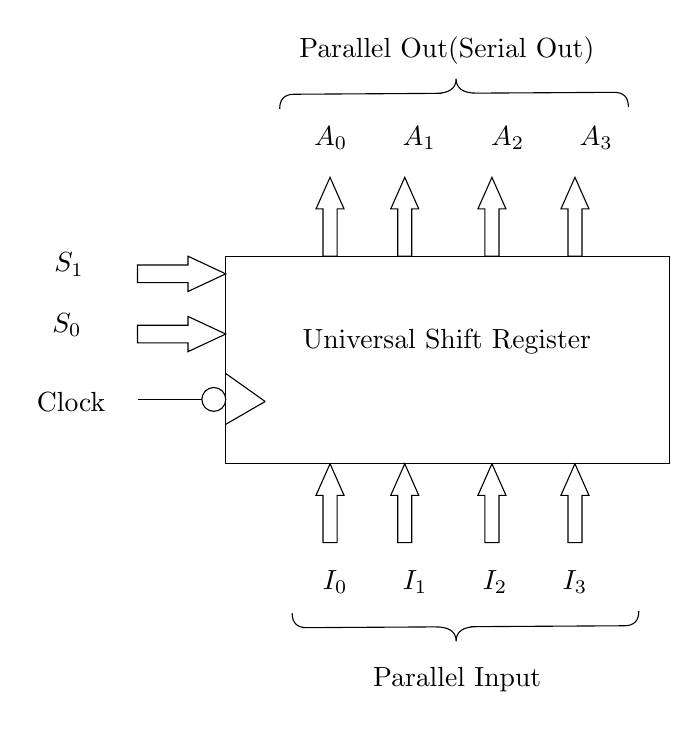
\begin{tikzpicture}[x=0.75pt,y=0.75pt,yscale=-1,xscale=1]
%uncomment if require: \path (0,379); %set diagram left start at 0, and has height of 379

\draw    (228.5, 113) rectangle (442.5, 213)   ;
\draw   (272,228.2) -- (278.75,213) -- (285.5,228.2) -- (282.13,228.2) -- (282.13,251) -- (275.38,251) -- (275.38,228.2) -- cycle ;
\draw   (308,228.2) -- (314.75,213) -- (321.5,228.2) -- (318.13,228.2) -- (318.13,251) -- (311.38,251) -- (311.38,228.2) -- cycle ;
\draw   (350,228.2) -- (356.75,213) -- (363.5,228.2) -- (360.13,228.2) -- (360.13,251) -- (353.38,251) -- (353.38,228.2) -- cycle ;
\draw   (390,228.2) -- (396.75,213) -- (403.5,228.2) -- (400.13,228.2) -- (400.13,251) -- (393.38,251) -- (393.38,228.2) -- cycle ;
\draw   (260.5,285) .. controls (260.53,289.67) and (262.87,291.99) .. (267.54,291.96) -- (329.46,291.59) .. controls (336.13,291.55) and (339.47,293.86) .. (339.5,298.53) .. controls (339.47,293.86) and (342.79,291.51) .. (349.46,291.47)(346.46,291.49) -- (420.54,291.05) .. controls (425.21,291.02) and (427.53,288.68) .. (427.5,284.01) ;
\draw   (272,90.2) -- (278.75,75) -- (285.5,90.2) -- (282.13,90.2) -- (282.13,113) -- (275.38,113) -- (275.38,90.2) -- cycle ;
\draw   (308,90.2) -- (314.75,75) -- (321.5,90.2) -- (318.13,90.2) -- (318.13,113) -- (311.38,113) -- (311.38,90.2) -- cycle ;
\draw   (350,90.2) -- (356.75,75) -- (363.5,90.2) -- (360.13,90.2) -- (360.13,113) -- (353.38,113) -- (353.38,90.2) -- cycle ;
\draw   (390,90.2) -- (396.75,75) -- (403.5,90.2) -- (400.13,90.2) -- (400.13,113) -- (393.38,113) -- (393.38,90.2) -- cycle ;
\draw   (422.5,41) .. controls (422.47,36.33) and (420.13,34.01) .. (415.46,34.04) -- (349.52,34.43) .. controls (342.85,34.47) and (339.51,32.16) .. (339.48,27.49) .. controls (339.51,32.16) and (336.19,34.51) .. (329.52,34.55)(332.52,34.53) -- (261.46,34.96) .. controls (256.79,34.99) and (254.47,37.33) .. (254.5,42) ;
\draw   (186,117.25) -- (210.3,117.25) -- (210.3,113) -- (228.5,121.5) -- (210.3,130) -- (210.3,125.75) -- (186,125.75) -- cycle ;
\draw   (186,146.25) -- (210.3,146.25) -- (210.3,142) -- (228.5,150.5) -- (210.3,159) -- (210.3,154.75) -- (186,154.75) -- cycle ;
\draw    (186,182) -- (217,182) ;


\draw    (222.75, 182) circle [x radius= 5.75, y radius= 5.75]  ;
\draw    (228.5,169.5) -- (247.5,183) ;


\draw    (247.5,183) -- (228.5,194) ;



\draw (335,14) node  [align=left] {Parallel Out(Serial Out)};
\draw (340,317) node  [align=left] {Parallel Input};
\draw (339,270) node  [align=left] {$I_0$ \ \ \ \ \  $I_1$ \ \ \ \ \ $I_2$ \ \ \ \ \ $I_3$};
\draw (343,56) node  [align=left] {$A_0$ \ \ \ \ \ $A_1$ \ \ \ \ \ $A_2$ \ \ \ \ \ $A_3$};
\draw (153,117) node   {$S_1$};
\draw (152,146) node   {$S_0$};
\draw (154,183) node  [align=left] {Clock};
\draw (335,154) node  [align=center] {Universal Shift Register};

\end{tikzpicture}
\label{fig:blockdiagram}
\caption{Block diagram of 4-bit universal shift register}
\end{figure}
In the 4-bit universal shift register,there are four parallel inputs and four parallel outputs,which can also be used for serial outputs.Universal shift register has a common clock that controls the built-in components such as D flip-flop.\\
There is two selection bits for a universal shift register.These two selection bits control the operations of a universal shift register.
\begin{table}[!h]
    \centering
    \begin{tabular}{|c|c|c|}
        \hline
         $S_1$ & $S_0$ & Register Operation\\ 
        \hline 
        0 & 0 & No change  \\
        \hline 
        0 & 1 & Shift Right  \\
        \hline 
        1 & 0 & Shift Left    \\
        \hline 
        1 & 1 & Parallel Load   \\
        \hline 
    \end{tabular}
    \caption{Operations of a universal shift register}
    \label{tab:selection}
\end{table}

\section{Components}
A universal shift register is basically constructed with two components. They are:
\begin{enumerate}
\item Multiplexer
\item D flip-flop
\end{enumerate}

\subsection{Multiplexer}
Multiplexer is a basic component of universal shift register.It is used for selecting the operations for the universal shift register.\\
\begin{figure}[!h]
    \centering
    \includegraphics[width=.8\textwidth]{pics/4to1mux.jpg}
    \caption{4 to 1 multiplexer}
    \label{fig:mux}
\end{figure}
In the following figure,we can see the basic circuit,block diagram and truth table of a 2 to 4 multiplexer.It has two selection bits $A$ and $B$ for selecting $D0,D1,D2,D3.$ 

Instead of the multiplexer, a 2 to 4 decoder can be used. \newpage
\subsection{D Flip-flop}
D flip-flop is used in universal shift register for storing data.It has a clock which controls the operations of the flip flop.\\
\begin{figure}[!h]
    \centering
    \includegraphics[width=.8\textwidth]{pics/flipflop.jpg}
    \caption{D Flip-flop}
    \label{fig:flip-flop}
\end{figure}
In this flip-flop, when clock is cleared that means $clock=0$,there is no effect of changing input data, $D$ on the output data,$Q$.But when is clock is changed to $1$,the output data,$Q$ will be followed by input data $D$.

A J-K flip-flop can be replaced with D flip-flop.\newpage
\section{Working Procedure}
In this section,we are going to discuss the working procedure of a universal shift register.\\
\begin{figure}[!ht]
    \centering
\tikzset{every picture/.style={line width=0.75pt}} %set default line width to 0.75pt        

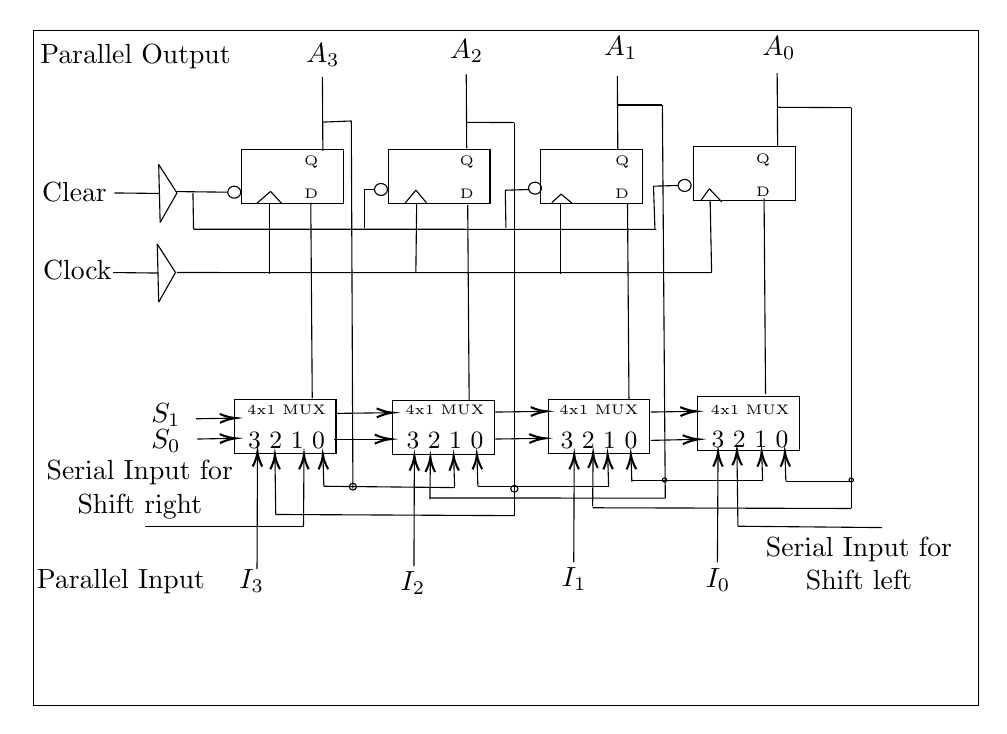
\begin{tikzpicture}[x=0.75pt,y=0.75pt,yscale=-.65,xscale=.7]
   \centering
%uncomment if require: \path (0,482.89410400390625); %set diagram left start at 0, and has height of 482.89410400390625
\draw (0,0) rectangle (650,500);
\draw    (247, 274) rectangle (317, 314)   ;
\draw    (138, 273) rectangle (208, 313)   ;
\draw    (354, 273) rectangle (424, 313)   ;
\draw    (457, 271) rectangle (527, 311)   ;
\draw    (244, 88) rectangle (314, 128)   ;
\draw    (143, 88) rectangle (213, 128)   ;
\draw    (349, 88) rectangle (419, 128)   ;
\draw    (454, 86) rectangle (524, 126)   ;
\draw    (111.68,287.53) -- (137,287.04) ;
\draw [shift={(139,287)}, rotate = 538.88] [color={rgb, 255:red, 0; green, 0; blue, 0 }  ][line width=0.75]    (10.93,-3.29) .. controls (6.95,-1.4) and (3.31,-0.3) .. (0,0) .. controls (3.31,0.3) and (6.95,1.4) .. (10.93,3.29)   ;

\draw    (112.68,302.53) -- (137,302.04) ;
\draw [shift={(139,302)}, rotate = 538.8399999999999] [color={rgb, 255:red, 0; green, 0; blue, 0 }  ][line width=0.75]    (10.93,-3.29) .. controls (6.95,-1.4) and (3.31,-0.3) .. (0,0) .. controls (3.31,0.3) and (6.95,1.4) .. (10.93,3.29)   ;

\draw    (153.68,398.85) -- (153.99,314) ;
\draw [shift={(154,312)}, rotate = 450.21] [color={rgb, 255:red, 0; green, 0; blue, 0 }  ][line width=0.75]    (10.93,-3.29) .. controls (6.95,-1.4) and (3.31,-0.3) .. (0,0) .. controls (3.31,0.3) and (6.95,1.4) .. (10.93,3.29)   ;

\draw    (261.68,396.85) -- (261.99,317) ;
\draw [shift={(262,315)}, rotate = 450.22] [color={rgb, 255:red, 0; green, 0; blue, 0 }  ][line width=0.75]    (10.93,-3.29) .. controls (6.95,-1.4) and (3.31,-0.3) .. (0,0) .. controls (3.31,0.3) and (6.95,1.4) .. (10.93,3.29)   ;

\draw    (371.68,393.85) -- (371.99,316) ;
\draw [shift={(372,314)}, rotate = 450.23] [color={rgb, 255:red, 0; green, 0; blue, 0 }  ][line width=0.75]    (10.93,-3.29) .. controls (6.95,-1.4) and (3.31,-0.3) .. (0,0) .. controls (3.31,0.3) and (6.95,1.4) .. (10.93,3.29)   ;

\draw    (470.56,393.89) -- (470.99,314) ;
\draw [shift={(471,312)}, rotate = 450.31] [color={rgb, 255:red, 0; green, 0; blue, 0 }  ][line width=0.75]    (10.93,-3.29) .. controls (6.95,-1.4) and (3.31,-0.3) .. (0,0) .. controls (3.31,0.3) and (6.95,1.4) .. (10.93,3.29)   ;

\draw    (185.68,367.16) -- (185.99,316) ;
\draw [shift={(186,314)}, rotate = 450.34] [color={rgb, 255:red, 0; green, 0; blue, 0 }  ][line width=0.75]    (10.93,-3.29) .. controls (6.95,-1.4) and (3.31,-0.3) .. (0,0) .. controls (3.31,0.3) and (6.95,1.4) .. (10.93,3.29)   ;

\draw    (76.68,367.16) -- (185.68,367.16) ;


\draw    (484.68,367.16) -- (484.02,313) ;
\draw [shift={(484,311)}, rotate = 449.3] [color={rgb, 255:red, 0; green, 0; blue, 0 }  ][line width=0.75]    (10.93,-3.29) .. controls (6.95,-1.4) and (3.31,-0.3) .. (0,0) .. controls (3.31,0.3) and (6.95,1.4) .. (10.93,3.29)   ;

\draw    (484.68,367.16) -- (583.68,368.16) ;


\draw    (511.68,31.27) -- (512,86) ;


\draw    (401.68,33.27) -- (402,88) ;


\draw    (297.68,32.27) -- (298,87) ;


\draw    (198.68,34.27) -- (199,89) ;


\draw    (562.68,56.9) -- (562.68,333.9) ;


\draw    (517.68,333.9) -- (562.68,333.9) ;


\draw    (511.84,56.63) -- (562.68,56.9) ;


\draw    (517.68,333.9) -- (517.06,314) ;
\draw [shift={(517,312)}, rotate = 448.21] [color={rgb, 255:red, 0; green, 0; blue, 0 }  ][line width=0.75]    (10.93,-3.29) .. controls (6.95,-1.4) and (3.31,-0.3) .. (0,0) .. controls (3.31,0.3) and (6.95,1.4) .. (10.93,3.29)   ;

\draw    (501.68,333.53) -- (501.06,314) ;
\draw [shift={(501,312)}, rotate = 448.18] [color={rgb, 255:red, 0; green, 0; blue, 0 }  ][line width=0.75]    (10.93,-3.29) .. controls (6.95,-1.4) and (3.31,-0.3) .. (0,0) .. controls (3.31,0.3) and (6.95,1.4) .. (10.93,3.29)   ;

\draw    (411.68,334.53) -- (411.07,316) ;
\draw [shift={(411,314)}, rotate = 448.09] [color={rgb, 255:red, 0; green, 0; blue, 0 }  ][line width=0.75]    (10.93,-3.29) .. controls (6.95,-1.4) and (3.31,-0.3) .. (0,0) .. controls (3.31,0.3) and (6.95,1.4) .. (10.93,3.29)   ;

\draw    (411.68,333.53) -- (501.68,333.53) ;


\draw    (562.68,354.01) -- (562.68,333.9) ;


\draw    (384.68,352.48) -- (384.98,315) ;
\draw [shift={(385,313)}, rotate = 450.46] [color={rgb, 255:red, 0; green, 0; blue, 0 }  ][line width=0.75]    (10.93,-3.29) .. controls (6.95,-1.4) and (3.31,-0.3) .. (0,0) .. controls (3.31,0.3) and (6.95,1.4) .. (10.93,3.29)   ;

\draw    (384.68,353.48) -- (562.68,354.01) ;


\draw    (305.68,337.53) -- (395.68,337.53) ;


\draw    (395.68,337.53) -- (395.06,316) ;
\draw [shift={(395,314)}, rotate = 448.33] [color={rgb, 255:red, 0; green, 0; blue, 0 }  ][line width=0.75]    (10.93,-3.29) .. controls (6.95,-1.4) and (3.31,-0.3) .. (0,0) .. controls (3.31,0.3) and (6.95,1.4) .. (10.93,3.29)   ;

\draw    (305.68,337.53) -- (305.06,316) ;
\draw [shift={(305,314)}, rotate = 448.33] [color={rgb, 255:red, 0; green, 0; blue, 0 }  ][line width=0.75]    (10.93,-3.29) .. controls (6.95,-1.4) and (3.31,-0.3) .. (0,0) .. controls (3.31,0.3) and (6.95,1.4) .. (10.93,3.29)   ;

\draw    (289.68,338.53) -- (289.06,317) ;
\draw [shift={(289,315)}, rotate = 448.33] [color={rgb, 255:red, 0; green, 0; blue, 0 }  ][line width=0.75]    (10.93,-3.29) .. controls (6.95,-1.4) and (3.31,-0.3) .. (0,0) .. controls (3.31,0.3) and (6.95,1.4) .. (10.93,3.29)   ;

\draw    (199.68,337.53) -- (199.06,316) ;
\draw [shift={(199,314)}, rotate = 448.33] [color={rgb, 255:red, 0; green, 0; blue, 0 }  ][line width=0.75]    (10.93,-3.29) .. controls (6.95,-1.4) and (3.31,-0.3) .. (0,0) .. controls (3.31,0.3) and (6.95,1.4) .. (10.93,3.29)   ;

\draw    (199.68,337.53) -- (289.68,338.53) ;


\draw    (502.68,124.22) -- (503.68,269.22) ;


\draw    (408.68,128.22) -- (409.68,273.22) ;


\draw    (298.68,129.22) -- (299.68,274.22) ;


\draw    (190.68,127.22) -- (191.68,272.22) ;


\draw    (206.68,302.59) -- (243.68,302.59) ;
\draw [shift={(245.68,302.59)}, rotate = 180] [color={rgb, 255:red, 0; green, 0; blue, 0 }  ][line width=0.75]    (10.93,-3.29) .. controls (6.95,-1.4) and (3.31,-0.3) .. (0,0) .. controls (3.31,0.3) and (6.95,1.4) .. (10.93,3.29)   ;

\draw    (317.68,302.53) -- (350,302.03) ;
\draw [shift={(352,302)}, rotate = 539.11] [color={rgb, 255:red, 0; green, 0; blue, 0 }  ][line width=0.75]    (10.93,-3.29) .. controls (6.95,-1.4) and (3.31,-0.3) .. (0,0) .. controls (3.31,0.3) and (6.95,1.4) .. (10.93,3.29)   ;

\draw    (424.68,303.53) -- (455.68,302.79) ;
\draw [shift={(457.68,302.74)}, rotate = 538.63] [color={rgb, 255:red, 0; green, 0; blue, 0 }  ][line width=0.75]    (10.93,-3.29) .. controls (6.95,-1.4) and (3.31,-0.3) .. (0,0) .. controls (3.31,0.3) and (6.95,1.4) .. (10.93,3.29)   ;

\draw    (208.68,283.53) -- (245,283.03) ;
\draw [shift={(247,283)}, rotate = 539.2] [color={rgb, 255:red, 0; green, 0; blue, 0 }  ][line width=0.75]    (10.93,-3.29) .. controls (6.95,-1.4) and (3.31,-0.3) .. (0,0) .. controls (3.31,0.3) and (6.95,1.4) .. (10.93,3.29)   ;

\draw    (317.68,282.53) -- (351,282.03) ;
\draw [shift={(353,282)}, rotate = 539.14] [color={rgb, 255:red, 0; green, 0; blue, 0 }  ][line width=0.75]    (10.93,-3.29) .. controls (6.95,-1.4) and (3.31,-0.3) .. (0,0) .. controls (3.31,0.3) and (6.95,1.4) .. (10.93,3.29)   ;

\draw    (424.68,282.53) -- (454,282.03) ;
\draw [shift={(456,282)}, rotate = 539.03] [color={rgb, 255:red, 0; green, 0; blue, 0 }  ][line width=0.75]    (10.93,-3.29) .. controls (6.95,-1.4) and (3.31,-0.3) .. (0,0) .. controls (3.31,0.3) and (6.95,1.4) .. (10.93,3.29)   ;

\draw    (272.68,347.22) -- (272.98,318) ;
\draw [shift={(273,316)}, rotate = 450.58] [color={rgb, 255:red, 0; green, 0; blue, 0 }  ][line width=0.75]    (10.93,-3.29) .. controls (6.95,-1.4) and (3.31,-0.3) .. (0,0) .. controls (3.31,0.3) and (6.95,1.4) .. (10.93,3.29)   ;

\draw    (434.68,346.32) -- (272.68,346.22) ;


\draw    (432.68,54.95) -- (434.68,346.32) ;


\draw    (401.68,54.95) -- (432.68,54.95) ;


\draw    (562.68, 332.9) circle [x radius= 1.5, y radius= 1.5]  ;
\draw    (434.18, 332.9) circle [x radius= 1.5, y radius= 1.5]  ;
\draw    (330.68,67.95) -- (330.68,359.32) ;


\draw    (166.56,358.45) -- (166.02,316) ;
\draw [shift={(166,314)}, rotate = 449.28] [color={rgb, 255:red, 0; green, 0; blue, 0 }  ][line width=0.75]    (10.93,-3.29) .. controls (6.95,-1.4) and (3.31,-0.3) .. (0,0) .. controls (3.31,0.3) and (6.95,1.4) .. (10.93,3.29)   ;

\draw    (166.56,358.45) -- (330.68,359.32) ;


\draw    (330.79, 339.39) circle [x radius= 2.5, y radius= 2.5]  ;
\draw    (297.56,67.78) -- (330.68,67.95) ;


\draw    (218.56,66.78) -- (219.68,339.32) ;


\draw    (198.84,67.63) -- (218.56,66.78) ;


\draw    (219.68, 337.84) circle [x radius= 2.5, y radius= 2.5]  ;
\draw    (55.56,120.12) -- (86.5,120.5) ;


\draw    (86,99) -- (98.56,120.12) ;


\draw    (87,142) -- (98.56,120.12) ;


\draw    (86,99) -- (87,142) ;


\draw    (138, 119.56) circle [x radius= 4.44, y radius= 4.44]  ;
\draw    (239, 117.56) circle [x radius= 4.44, y radius= 4.44]  ;
\draw    (345, 116.56) circle [x radius= 4.44, y radius= 4.44]  ;
\draw    (448, 114.56) circle [x radius= 4.44, y radius= 4.44]  ;
\draw    (98.56,119.12) -- (133.56,119.56) ;


\draw    (110,147) -- (428.56,147.12) ;


\draw    (110,147) -- (109.56,120.12) ;


\draw    (227.56,117.56) -- (227.56,146.12) ;


\draw    (227.56,117.56) -- (234.56,117.56) ;


\draw    (325,146) -- (324.56,118.12) ;


\draw    (324.56,118.12) -- (340.56,117.56) ;


\draw    (427.56,147.12) -- (426.56,115.12) ;


\draw    (426.56,115.12) -- (443.56,114.56) ;


\draw    (54.56,179.12) -- (85.5,179.5) ;


\draw    (85,158) -- (97.56,179.12) ;


\draw    (86,201) -- (97.56,179.12) ;


\draw    (85,158) -- (86,201) ;


\draw    (98.56,179.12) -- (466.56,179.23) ;


%\draw    (102.56, 179.12) circle [x radius= 5, y radius= 5]  ;
\draw    (465.56,125.23) -- (466.56,179.23) ;


\draw    (362.56,127.23) -- (362.56,180.23) ;


\draw    (263.56,128.23) -- (263,179) ;


\draw    (162,128) -- (162,180) ;


\draw    (163,119) -- (170.56,127.78) ;


\draw    (163,119) -- (153.56,127.78) ;


\draw    (263,118) -- (270.56,127.78) ;


\draw    (263,118) -- (255.56,127.78) ;


\draw    (363,121) -- (370.56,127.78) ;


\draw    (363,121) -- (356.56,127.23) ;


\draw    (465,117) -- (473.56,126.78) ;


\draw    (465,117) -- (459,126) ;



\draw (150,408) node  [align=center] {$I_3$};
\draw (261,409) node  [align=center] {$I_2$};
\draw (372,406) node [align=center]{$I_1$};
\draw (471,407) node [align=center] {$I_0$};
\draw (73,340) node  [align=center] {Serial Input for\\Shift right};
\draw (568,395) node  [align=center] {Serial Input for\\Shift left};
\draw (91,285) node  [align=center] {$S_1$};
\draw (91,304) node [align=center] {$S_0$};
\draw (199,18) node  [align=center] {$A_3$};
\draw (298,15) node  [align=center] {$A_2$};
\draw (404,13) node  [align=center] {$A_1$};
\draw (513,13) node  [align=center] {$A_0$};
\draw (60,408) node  [align=center] {Parallel Input};
\draw (70,19) node  [align=center] {Parallel Output};
\draw (28,119) node  [align=center] {Clear};
\draw (30,177) node  [align=center] {Clock};
\draw (191,108.5) node  [align=center] {\tiny Q\\\tiny D};
\draw (298,108.5) node  [align=center] {\tiny Q\\\tiny D};
\draw (405,108.5) node  [align=center] {\tiny Q\\\tiny D};
\draw (502,107) node  [align=center] {\tiny Q\\\tiny D};
\draw (174,293.5) node [align=center] {\tiny 4x1 MUX\\\small 3 2 1 0};
\draw (283,293.5) node  [align=center] {\tiny 4x1 MUX\\\small 3 2 1 0};
\draw (389,293.5) node  [align=center] {\tiny 4x1 MUX\\\small 3 2 1 0};
\draw (493,293) node  [align=center] {\tiny 4x1 MUX\\\small 3 2 1 0};


\end{tikzpicture}
    \caption{Circuit diagram of universal shift register}
    \label{fig:circuit}
\end{figure}
In the following figure, we can see the circuit diagram of a 4-bit universal shift register. There are four parallel inputs and four serial outputs.Two inputs for selection bits and input for serial input for serial left and right.There is also a common clock and clear option for four D flip-flops.
\subsection{Storing Data}
Universal shift register can be used as storing data.When $S_1=0$ and $S_0=0$ the outputs of the universal shift register will not change.\newpage
\begin{figure}[!ht]
    \centering
\tikzset{every picture/.style={line width=0.75pt}} %set default line width to 0.75pt        

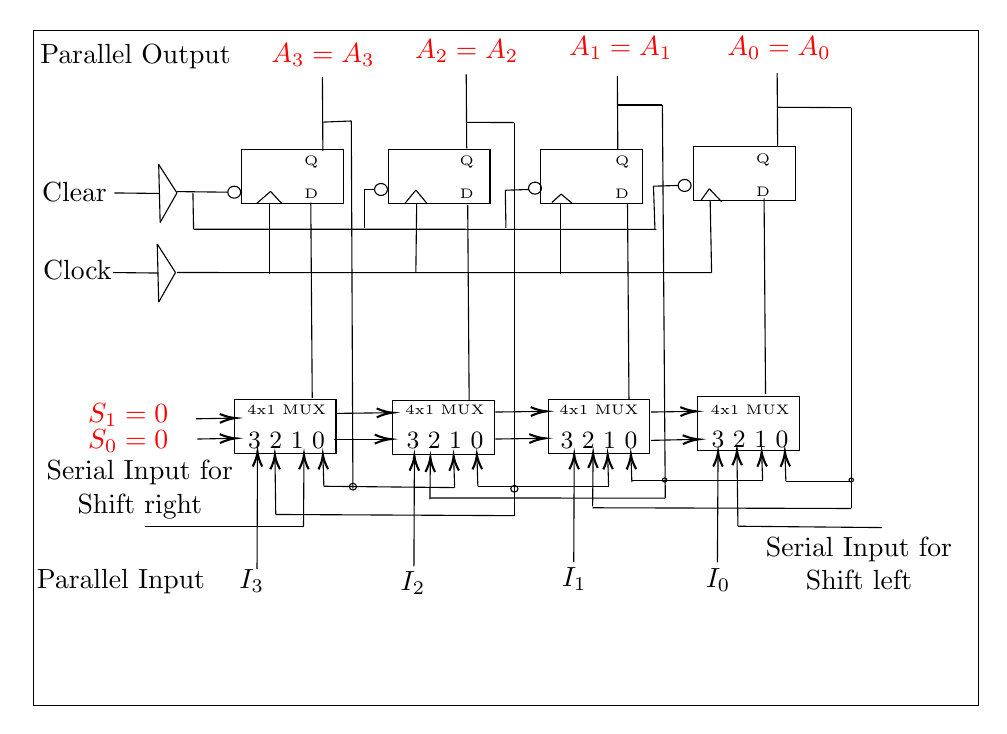
\begin{tikzpicture}[x=0.75pt,y=0.75pt,yscale=-.65,xscale=.7]
   \centering
%uncomment if require: \path (0,482.89410400390625); %set diagram left start at 0, and has height of 482.89410400390625
\draw (0,0) rectangle (650,500);
\draw    (247, 274) rectangle (317, 314)   ;
\draw    (138, 273) rectangle (208, 313)   ;
\draw    (354, 273) rectangle (424, 313)   ;
\draw    (457, 271) rectangle (527, 311)   ;
\draw    (244, 88) rectangle (314, 128)   ;
\draw    (143, 88) rectangle (213, 128)   ;
\draw    (349, 88) rectangle (419, 128)   ;
\draw    (454, 86) rectangle (524, 126)   ;
\draw    (111.68,287.53) -- (137,287.04) ;
\draw [shift={(139,287)}, rotate = 538.88] [color={rgb, 255:red, 0; green, 0; blue, 0 }  ][line width=0.75]    (10.93,-3.29) .. controls (6.95,-1.4) and (3.31,-0.3) .. (0,0) .. controls (3.31,0.3) and (6.95,1.4) .. (10.93,3.29)   ;

\draw    (112.68,302.53) -- (137,302.04) ;
\draw [shift={(139,302)}, rotate = 538.8399999999999] [color={rgb, 255:red, 0; green, 0; blue, 0 }  ][line width=0.75]    (10.93,-3.29) .. controls (6.95,-1.4) and (3.31,-0.3) .. (0,0) .. controls (3.31,0.3) and (6.95,1.4) .. (10.93,3.29)   ;

\draw    (153.68,398.85) -- (153.99,314) ;
\draw [shift={(154,312)}, rotate = 450.21] [color={rgb, 255:red, 0; green, 0; blue, 0 }  ][line width=0.75]    (10.93,-3.29) .. controls (6.95,-1.4) and (3.31,-0.3) .. (0,0) .. controls (3.31,0.3) and (6.95,1.4) .. (10.93,3.29)   ;

\draw    (261.68,396.85) -- (261.99,317) ;
\draw [shift={(262,315)}, rotate = 450.22] [color={rgb, 255:red, 0; green, 0; blue, 0 }  ][line width=0.75]    (10.93,-3.29) .. controls (6.95,-1.4) and (3.31,-0.3) .. (0,0) .. controls (3.31,0.3) and (6.95,1.4) .. (10.93,3.29)   ;

\draw    (371.68,393.85) -- (371.99,316) ;
\draw [shift={(372,314)}, rotate = 450.23] [color={rgb, 255:red, 0; green, 0; blue, 0 }  ][line width=0.75]    (10.93,-3.29) .. controls (6.95,-1.4) and (3.31,-0.3) .. (0,0) .. controls (3.31,0.3) and (6.95,1.4) .. (10.93,3.29)   ;

\draw    (470.56,393.89) -- (470.99,314) ;
\draw [shift={(471,312)}, rotate = 450.31] [color={rgb, 255:red, 0; green, 0; blue, 0 }  ][line width=0.75]    (10.93,-3.29) .. controls (6.95,-1.4) and (3.31,-0.3) .. (0,0) .. controls (3.31,0.3) and (6.95,1.4) .. (10.93,3.29)   ;

\draw    (185.68,367.16) -- (185.99,316) ;
\draw [shift={(186,314)}, rotate = 450.34] [color={rgb, 255:red, 0; green, 0; blue, 0 }  ][line width=0.75]    (10.93,-3.29) .. controls (6.95,-1.4) and (3.31,-0.3) .. (0,0) .. controls (3.31,0.3) and (6.95,1.4) .. (10.93,3.29)   ;

\draw    (76.68,367.16) -- (185.68,367.16) ;


\draw    (484.68,367.16) -- (484.02,313) ;
\draw [shift={(484,311)}, rotate = 449.3] [color={rgb, 255:red, 0; green, 0; blue, 0 }  ][line width=0.75]    (10.93,-3.29) .. controls (6.95,-1.4) and (3.31,-0.3) .. (0,0) .. controls (3.31,0.3) and (6.95,1.4) .. (10.93,3.29)   ;

\draw    (484.68,367.16) -- (583.68,368.16) ;


\draw    (511.68,31.27) -- (512,86) ;


\draw    (401.68,33.27) -- (402,88) ;


\draw    (297.68,32.27) -- (298,87) ;


\draw    (198.68,34.27) -- (199,89) ;


\draw    (562.68,56.9) -- (562.68,333.9) ;


\draw    (517.68,333.9) -- (562.68,333.9) ;


\draw    (511.84,56.63) -- (562.68,56.9) ;


\draw    (517.68,333.9) -- (517.06,314) ;
\draw [shift={(517,312)}, rotate = 448.21] [color={rgb, 255:red, 0; green, 0; blue, 0 }  ][line width=0.75]    (10.93,-3.29) .. controls (6.95,-1.4) and (3.31,-0.3) .. (0,0) .. controls (3.31,0.3) and (6.95,1.4) .. (10.93,3.29)   ;

\draw    (501.68,333.53) -- (501.06,314) ;
\draw [shift={(501,312)}, rotate = 448.18] [color={rgb, 255:red, 0; green, 0; blue, 0 }  ][line width=0.75]    (10.93,-3.29) .. controls (6.95,-1.4) and (3.31,-0.3) .. (0,0) .. controls (3.31,0.3) and (6.95,1.4) .. (10.93,3.29)   ;

\draw    (411.68,334.53) -- (411.07,316) ;
\draw [shift={(411,314)}, rotate = 448.09] [color={rgb, 255:red, 0; green, 0; blue, 0 }  ][line width=0.75]    (10.93,-3.29) .. controls (6.95,-1.4) and (3.31,-0.3) .. (0,0) .. controls (3.31,0.3) and (6.95,1.4) .. (10.93,3.29)   ;

\draw    (411.68,333.53) -- (501.68,333.53) ;


\draw    (562.68,354.01) -- (562.68,333.9) ;


\draw    (384.68,352.48) -- (384.98,315) ;
\draw [shift={(385,313)}, rotate = 450.46] [color={rgb, 255:red, 0; green, 0; blue, 0 }  ][line width=0.75]    (10.93,-3.29) .. controls (6.95,-1.4) and (3.31,-0.3) .. (0,0) .. controls (3.31,0.3) and (6.95,1.4) .. (10.93,3.29)   ;

\draw    (384.68,353.48) -- (562.68,354.01) ;


\draw    (305.68,337.53) -- (395.68,337.53) ;


\draw    (395.68,337.53) -- (395.06,316) ;
\draw [shift={(395,314)}, rotate = 448.33] [color={rgb, 255:red, 0; green, 0; blue, 0 }  ][line width=0.75]    (10.93,-3.29) .. controls (6.95,-1.4) and (3.31,-0.3) .. (0,0) .. controls (3.31,0.3) and (6.95,1.4) .. (10.93,3.29)   ;

\draw    (305.68,337.53) -- (305.06,316) ;
\draw [shift={(305,314)}, rotate = 448.33] [color={rgb, 255:red, 0; green, 0; blue, 0 }  ][line width=0.75]    (10.93,-3.29) .. controls (6.95,-1.4) and (3.31,-0.3) .. (0,0) .. controls (3.31,0.3) and (6.95,1.4) .. (10.93,3.29)   ;

\draw    (289.68,338.53) -- (289.06,317) ;
\draw [shift={(289,315)}, rotate = 448.33] [color={rgb, 255:red, 0; green, 0; blue, 0 }  ][line width=0.75]    (10.93,-3.29) .. controls (6.95,-1.4) and (3.31,-0.3) .. (0,0) .. controls (3.31,0.3) and (6.95,1.4) .. (10.93,3.29)   ;

\draw    (199.68,337.53) -- (199.06,316) ;
\draw [shift={(199,314)}, rotate = 448.33] [color={rgb, 255:red, 0; green, 0; blue, 0 }  ][line width=0.75]    (10.93,-3.29) .. controls (6.95,-1.4) and (3.31,-0.3) .. (0,0) .. controls (3.31,0.3) and (6.95,1.4) .. (10.93,3.29)   ;

\draw    (199.68,337.53) -- (289.68,338.53) ;


\draw    (502.68,124.22) -- (503.68,269.22) ;


\draw    (408.68,128.22) -- (409.68,273.22) ;


\draw    (298.68,129.22) -- (299.68,274.22) ;


\draw    (190.68,127.22) -- (191.68,272.22) ;


\draw    (206.68,302.59) -- (243.68,302.59) ;
\draw [shift={(245.68,302.59)}, rotate = 180] [color={rgb, 255:red, 0; green, 0; blue, 0 }  ][line width=0.75]    (10.93,-3.29) .. controls (6.95,-1.4) and (3.31,-0.3) .. (0,0) .. controls (3.31,0.3) and (6.95,1.4) .. (10.93,3.29)   ;

\draw    (317.68,302.53) -- (350,302.03) ;
\draw [shift={(352,302)}, rotate = 539.11] [color={rgb, 255:red, 0; green, 0; blue, 0 }  ][line width=0.75]    (10.93,-3.29) .. controls (6.95,-1.4) and (3.31,-0.3) .. (0,0) .. controls (3.31,0.3) and (6.95,1.4) .. (10.93,3.29)   ;

\draw    (424.68,303.53) -- (455.68,302.79) ;
\draw [shift={(457.68,302.74)}, rotate = 538.63] [color={rgb, 255:red, 0; green, 0; blue, 0 }  ][line width=0.75]    (10.93,-3.29) .. controls (6.95,-1.4) and (3.31,-0.3) .. (0,0) .. controls (3.31,0.3) and (6.95,1.4) .. (10.93,3.29)   ;

\draw    (208.68,283.53) -- (245,283.03) ;
\draw [shift={(247,283)}, rotate = 539.2] [color={rgb, 255:red, 0; green, 0; blue, 0 }  ][line width=0.75]    (10.93,-3.29) .. controls (6.95,-1.4) and (3.31,-0.3) .. (0,0) .. controls (3.31,0.3) and (6.95,1.4) .. (10.93,3.29)   ;

\draw    (317.68,282.53) -- (351,282.03) ;
\draw [shift={(353,282)}, rotate = 539.14] [color={rgb, 255:red, 0; green, 0; blue, 0 }  ][line width=0.75]    (10.93,-3.29) .. controls (6.95,-1.4) and (3.31,-0.3) .. (0,0) .. controls (3.31,0.3) and (6.95,1.4) .. (10.93,3.29)   ;

\draw    (424.68,282.53) -- (454,282.03) ;
\draw [shift={(456,282)}, rotate = 539.03] [color={rgb, 255:red, 0; green, 0; blue, 0 }  ][line width=0.75]    (10.93,-3.29) .. controls (6.95,-1.4) and (3.31,-0.3) .. (0,0) .. controls (3.31,0.3) and (6.95,1.4) .. (10.93,3.29)   ;

\draw    (272.68,347.22) -- (272.98,318) ;
\draw [shift={(273,316)}, rotate = 450.58] [color={rgb, 255:red, 0; green, 0; blue, 0 }  ][line width=0.75]    (10.93,-3.29) .. controls (6.95,-1.4) and (3.31,-0.3) .. (0,0) .. controls (3.31,0.3) and (6.95,1.4) .. (10.93,3.29)   ;

\draw    (434.68,346.32) -- (272.68,346.22) ;


\draw    (432.68,54.95) -- (434.68,346.32) ;


\draw    (401.68,54.95) -- (432.68,54.95) ;


\draw    (562.68, 332.9) circle [x radius= 1.5, y radius= 1.5]  ;
\draw    (434.18, 332.9) circle [x radius= 1.5, y radius= 1.5]  ;
\draw    (330.68,67.95) -- (330.68,359.32) ;


\draw    (166.56,358.45) -- (166.02,316) ;
\draw [shift={(166,314)}, rotate = 449.28] [color={rgb, 255:red, 0; green, 0; blue, 0 }  ][line width=0.75]    (10.93,-3.29) .. controls (6.95,-1.4) and (3.31,-0.3) .. (0,0) .. controls (3.31,0.3) and (6.95,1.4) .. (10.93,3.29)   ;

\draw    (166.56,358.45) -- (330.68,359.32) ;


\draw    (330.79, 339.39) circle [x radius= 2.5, y radius= 2.5]  ;
\draw    (297.56,67.78) -- (330.68,67.95) ;


\draw    (218.56,66.78) -- (219.68,339.32) ;


\draw    (198.84,67.63) -- (218.56,66.78) ;


\draw    (219.68, 337.84) circle [x radius= 2.5, y radius= 2.5]  ;
\draw    (55.56,120.12) -- (86.5,120.5) ;


\draw    (86,99) -- (98.56,120.12) ;


\draw    (87,142) -- (98.56,120.12) ;


\draw    (86,99) -- (87,142) ;


\draw    (138, 119.56) circle [x radius= 4.44, y radius= 4.44]  ;
\draw    (239, 117.56) circle [x radius= 4.44, y radius= 4.44]  ;
\draw    (345, 116.56) circle [x radius= 4.44, y radius= 4.44]  ;
\draw    (448, 114.56) circle [x radius= 4.44, y radius= 4.44]  ;
\draw    (98.56,119.12) -- (133.56,119.56) ;


\draw    (110,147) -- (428.56,147.12) ;


\draw    (110,147) -- (109.56,120.12) ;


\draw    (227.56,117.56) -- (227.56,146.12) ;


\draw    (227.56,117.56) -- (234.56,117.56) ;


\draw    (325,146) -- (324.56,118.12) ;


\draw    (324.56,118.12) -- (340.56,117.56) ;


\draw    (427.56,147.12) -- (426.56,115.12) ;


\draw    (426.56,115.12) -- (443.56,114.56) ;


\draw    (54.56,179.12) -- (85.5,179.5) ;


\draw    (85,158) -- (97.56,179.12) ;


\draw    (86,201) -- (97.56,179.12) ;


\draw    (85,158) -- (86,201) ;


\draw    (98.56,179.12) -- (466.56,179.23) ;


%\draw    (102.56, 179.12) circle [x radius= 5, y radius= 5]  ;
\draw    (465.56,125.23) -- (466.56,179.23) ;


\draw    (362.56,127.23) -- (362.56,180.23) ;


\draw    (263.56,128.23) -- (263,179) ;


\draw    (162,128) -- (162,180) ;


\draw    (163,119) -- (170.56,127.78) ;


\draw    (163,119) -- (153.56,127.78) ;


\draw    (263,118) -- (270.56,127.78) ;


\draw    (263,118) -- (255.56,127.78) ;


\draw    (363,121) -- (370.56,127.78) ;


\draw    (363,121) -- (356.56,127.23) ;


\draw    (465,117) -- (473.56,126.78) ;


\draw    (465,117) -- (459,126) ;



\draw (150,408) node  [align=center] {$I_3$};
\draw (261,409) node  [align=center] {$I_2$};
\draw (372,406) node [align=center]{$I_1$};
\draw (471,407) node [align=center] {$I_0$};
\draw (73,340) node  [align=center] {Serial Input for\\Shift right};
\draw (568,395) node  [align=center] {Serial Input for\\Shift left};
\draw (65,285) node  [align=center,color=red] {$S_1=0$};
\draw (65,304) node [align=center,color=red] {$S_0=0$};
\draw (199,18) node  [align=center,color=red] {$A_3=A_3$};
\draw (298,15) node  [align=center,color=red] {$A_2=A_2$};
\draw (404,13) node  [align=center,color=red] {$A_1=A_1$};
\draw (513,13) node  [align=center,color=red] {$A_0=A_0$};
\draw (60,408) node  [align=center] {Parallel Input};
\draw (70,19) node  [align=center] {Parallel Output};
\draw (28,119) node  [align=center] {Clear};
\draw (30,177) node  [align=center] {Clock};
\draw (191,108.5) node  [align=center] {\tiny Q\\\tiny D};
\draw (298,108.5) node  [align=center] {\tiny Q\\\tiny D};
\draw (405,108.5) node  [align=center] {\tiny Q\\\tiny D};
\draw (502,107) node  [align=center] {\tiny Q\\\tiny D};
\draw (174,293.5) node [align=center] {\tiny 4x1 MUX\\\small 3 2 1 0};
\draw (283,293.5) node  [align=center] {\tiny 4x1 MUX\\\small 3 2 1 0};
\draw (389,293.5) node  [align=center] {\tiny 4x1 MUX\\\small 3 2 1 0};
\draw (493,293) node  [align=center] {\tiny 4x1 MUX\\\small 3 2 1 0};


\end{tikzpicture}
    \caption{Storing data by universal shift register}
    \label{fig:store}
\end{figure}
We can see from the figure that,outputs of the universal shift register will not be effected if selection bits, $S_1=0$ and $S_0=0$.This configuration can be used to store information for different purposes in electrical devices.
\subsection{Right Shifting}
We can shift data to right by universal shift register.When $S_1=0$ and $S_0=1$ the outputs of the universal shift register will be shifted right and the last bit will take data from \textbf{serial input for shift right}.\newpage
\begin{figure}[!ht]
    \centering
\tikzset{every picture/.style={line width=0.75pt}} %set default line width to 0.75pt        

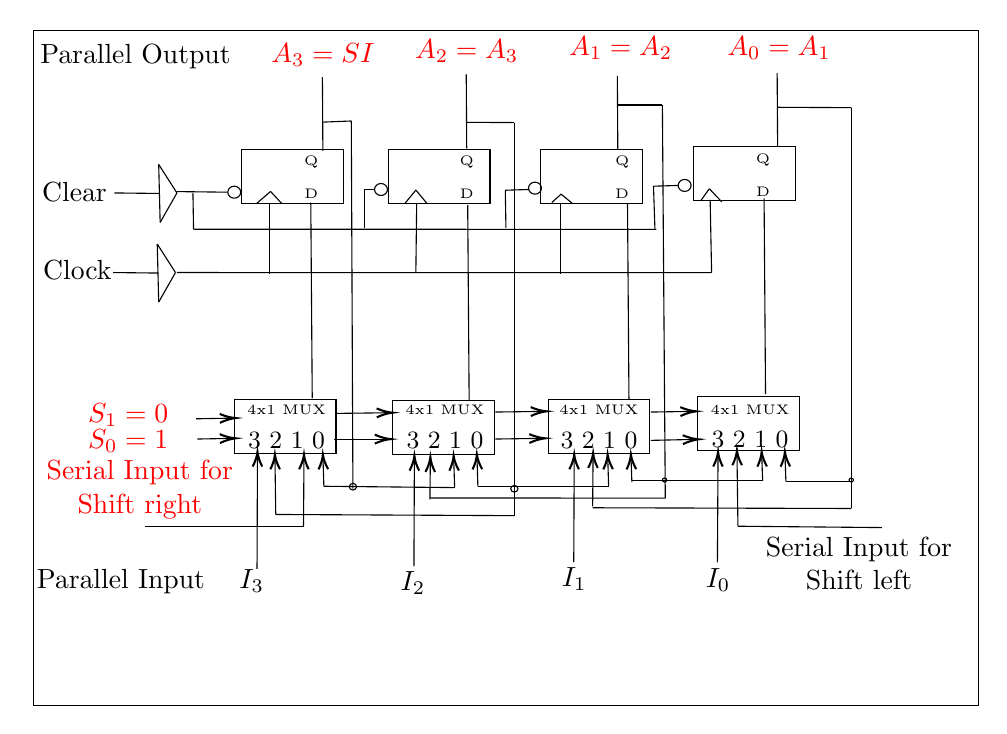
\begin{tikzpicture}[x=0.75pt,y=0.75pt,yscale=-.65,xscale=.7]
   \centering
%uncomment if require: \path (0,482.89410400390625); %set diagram left start at 0, and has height of 482.89410400390625
\draw (0,0) rectangle (650,500);
\draw    (247, 274) rectangle (317, 314)   ;
\draw    (138, 273) rectangle (208, 313)   ;
\draw    (354, 273) rectangle (424, 313)   ;
\draw    (457, 271) rectangle (527, 311)   ;
\draw    (244, 88) rectangle (314, 128)   ;
\draw    (143, 88) rectangle (213, 128)   ;
\draw    (349, 88) rectangle (419, 128)   ;
\draw    (454, 86) rectangle (524, 126)   ;
\draw    (111.68,287.53) -- (137,287.04) ;
\draw [shift={(139,287)}, rotate = 538.88] [color={rgb, 255:red, 0; green, 0; blue, 0 }  ][line width=0.75]    (10.93,-3.29) .. controls (6.95,-1.4) and (3.31,-0.3) .. (0,0) .. controls (3.31,0.3) and (6.95,1.4) .. (10.93,3.29)   ;

\draw    (112.68,302.53) -- (137,302.04) ;
\draw [shift={(139,302)}, rotate = 538.8399999999999] [color={rgb, 255:red, 0; green, 0; blue, 0 }  ][line width=0.75]    (10.93,-3.29) .. controls (6.95,-1.4) and (3.31,-0.3) .. (0,0) .. controls (3.31,0.3) and (6.95,1.4) .. (10.93,3.29)   ;

\draw    (153.68,398.85) -- (153.99,314) ;
\draw [shift={(154,312)}, rotate = 450.21] [color={rgb, 255:red, 0; green, 0; blue, 0 }  ][line width=0.75]    (10.93,-3.29) .. controls (6.95,-1.4) and (3.31,-0.3) .. (0,0) .. controls (3.31,0.3) and (6.95,1.4) .. (10.93,3.29)   ;

\draw    (261.68,396.85) -- (261.99,317) ;
\draw [shift={(262,315)}, rotate = 450.22] [color={rgb, 255:red, 0; green, 0; blue, 0 }  ][line width=0.75]    (10.93,-3.29) .. controls (6.95,-1.4) and (3.31,-0.3) .. (0,0) .. controls (3.31,0.3) and (6.95,1.4) .. (10.93,3.29)   ;

\draw    (371.68,393.85) -- (371.99,316) ;
\draw [shift={(372,314)}, rotate = 450.23] [color={rgb, 255:red, 0; green, 0; blue, 0 }  ][line width=0.75]    (10.93,-3.29) .. controls (6.95,-1.4) and (3.31,-0.3) .. (0,0) .. controls (3.31,0.3) and (6.95,1.4) .. (10.93,3.29)   ;

\draw    (470.56,393.89) -- (470.99,314) ;
\draw [shift={(471,312)}, rotate = 450.31] [color={rgb, 255:red, 0; green, 0; blue, 0 }  ][line width=0.75]    (10.93,-3.29) .. controls (6.95,-1.4) and (3.31,-0.3) .. (0,0) .. controls (3.31,0.3) and (6.95,1.4) .. (10.93,3.29)   ;

\draw    (185.68,367.16) -- (185.99,316) ;
\draw [shift={(186,314)}, rotate = 450.34] [color={rgb, 255:red, 0; green, 0; blue, 0 }  ][line width=0.75]    (10.93,-3.29) .. controls (6.95,-1.4) and (3.31,-0.3) .. (0,0) .. controls (3.31,0.3) and (6.95,1.4) .. (10.93,3.29)   ;

\draw    (76.68,367.16) -- (185.68,367.16) ;


\draw    (484.68,367.16) -- (484.02,313) ;
\draw [shift={(484,311)}, rotate = 449.3] [color={rgb, 255:red, 0; green, 0; blue, 0 }  ][line width=0.75]    (10.93,-3.29) .. controls (6.95,-1.4) and (3.31,-0.3) .. (0,0) .. controls (3.31,0.3) and (6.95,1.4) .. (10.93,3.29)   ;

\draw    (484.68,367.16) -- (583.68,368.16) ;


\draw    (511.68,31.27) -- (512,86) ;


\draw    (401.68,33.27) -- (402,88) ;


\draw    (297.68,32.27) -- (298,87) ;


\draw    (198.68,34.27) -- (199,89) ;


\draw    (562.68,56.9) -- (562.68,333.9) ;


\draw    (517.68,333.9) -- (562.68,333.9) ;


\draw    (511.84,56.63) -- (562.68,56.9) ;


\draw    (517.68,333.9) -- (517.06,314) ;
\draw [shift={(517,312)}, rotate = 448.21] [color={rgb, 255:red, 0; green, 0; blue, 0 }  ][line width=0.75]    (10.93,-3.29) .. controls (6.95,-1.4) and (3.31,-0.3) .. (0,0) .. controls (3.31,0.3) and (6.95,1.4) .. (10.93,3.29)   ;

\draw    (501.68,333.53) -- (501.06,314) ;
\draw [shift={(501,312)}, rotate = 448.18] [color={rgb, 255:red, 0; green, 0; blue, 0 }  ][line width=0.75]    (10.93,-3.29) .. controls (6.95,-1.4) and (3.31,-0.3) .. (0,0) .. controls (3.31,0.3) and (6.95,1.4) .. (10.93,3.29)   ;

\draw    (411.68,334.53) -- (411.07,316) ;
\draw [shift={(411,314)}, rotate = 448.09] [color={rgb, 255:red, 0; green, 0; blue, 0 }  ][line width=0.75]    (10.93,-3.29) .. controls (6.95,-1.4) and (3.31,-0.3) .. (0,0) .. controls (3.31,0.3) and (6.95,1.4) .. (10.93,3.29)   ;

\draw    (411.68,333.53) -- (501.68,333.53) ;


\draw    (562.68,354.01) -- (562.68,333.9) ;


\draw    (384.68,352.48) -- (384.98,315) ;
\draw [shift={(385,313)}, rotate = 450.46] [color={rgb, 255:red, 0; green, 0; blue, 0 }  ][line width=0.75]    (10.93,-3.29) .. controls (6.95,-1.4) and (3.31,-0.3) .. (0,0) .. controls (3.31,0.3) and (6.95,1.4) .. (10.93,3.29)   ;

\draw    (384.68,353.48) -- (562.68,354.01) ;


\draw    (305.68,337.53) -- (395.68,337.53) ;


\draw    (395.68,337.53) -- (395.06,316) ;
\draw [shift={(395,314)}, rotate = 448.33] [color={rgb, 255:red, 0; green, 0; blue, 0 }  ][line width=0.75]    (10.93,-3.29) .. controls (6.95,-1.4) and (3.31,-0.3) .. (0,0) .. controls (3.31,0.3) and (6.95,1.4) .. (10.93,3.29)   ;

\draw    (305.68,337.53) -- (305.06,316) ;
\draw [shift={(305,314)}, rotate = 448.33] [color={rgb, 255:red, 0; green, 0; blue, 0 }  ][line width=0.75]    (10.93,-3.29) .. controls (6.95,-1.4) and (3.31,-0.3) .. (0,0) .. controls (3.31,0.3) and (6.95,1.4) .. (10.93,3.29)   ;

\draw    (289.68,338.53) -- (289.06,317) ;
\draw [shift={(289,315)}, rotate = 448.33] [color={rgb, 255:red, 0; green, 0; blue, 0 }  ][line width=0.75]    (10.93,-3.29) .. controls (6.95,-1.4) and (3.31,-0.3) .. (0,0) .. controls (3.31,0.3) and (6.95,1.4) .. (10.93,3.29)   ;

\draw    (199.68,337.53) -- (199.06,316) ;
\draw [shift={(199,314)}, rotate = 448.33] [color={rgb, 255:red, 0; green, 0; blue, 0 }  ][line width=0.75]    (10.93,-3.29) .. controls (6.95,-1.4) and (3.31,-0.3) .. (0,0) .. controls (3.31,0.3) and (6.95,1.4) .. (10.93,3.29)   ;

\draw    (199.68,337.53) -- (289.68,338.53) ;


\draw    (502.68,124.22) -- (503.68,269.22) ;


\draw    (408.68,128.22) -- (409.68,273.22) ;


\draw    (298.68,129.22) -- (299.68,274.22) ;


\draw    (190.68,127.22) -- (191.68,272.22) ;


\draw    (206.68,302.59) -- (243.68,302.59) ;
\draw [shift={(245.68,302.59)}, rotate = 180] [color={rgb, 255:red, 0; green, 0; blue, 0 }  ][line width=0.75]    (10.93,-3.29) .. controls (6.95,-1.4) and (3.31,-0.3) .. (0,0) .. controls (3.31,0.3) and (6.95,1.4) .. (10.93,3.29)   ;

\draw    (317.68,302.53) -- (350,302.03) ;
\draw [shift={(352,302)}, rotate = 539.11] [color={rgb, 255:red, 0; green, 0; blue, 0 }  ][line width=0.75]    (10.93,-3.29) .. controls (6.95,-1.4) and (3.31,-0.3) .. (0,0) .. controls (3.31,0.3) and (6.95,1.4) .. (10.93,3.29)   ;

\draw    (424.68,303.53) -- (455.68,302.79) ;
\draw [shift={(457.68,302.74)}, rotate = 538.63] [color={rgb, 255:red, 0; green, 0; blue, 0 }  ][line width=0.75]    (10.93,-3.29) .. controls (6.95,-1.4) and (3.31,-0.3) .. (0,0) .. controls (3.31,0.3) and (6.95,1.4) .. (10.93,3.29)   ;

\draw    (208.68,283.53) -- (245,283.03) ;
\draw [shift={(247,283)}, rotate = 539.2] [color={rgb, 255:red, 0; green, 0; blue, 0 }  ][line width=0.75]    (10.93,-3.29) .. controls (6.95,-1.4) and (3.31,-0.3) .. (0,0) .. controls (3.31,0.3) and (6.95,1.4) .. (10.93,3.29)   ;

\draw    (317.68,282.53) -- (351,282.03) ;
\draw [shift={(353,282)}, rotate = 539.14] [color={rgb, 255:red, 0; green, 0; blue, 0 }  ][line width=0.75]    (10.93,-3.29) .. controls (6.95,-1.4) and (3.31,-0.3) .. (0,0) .. controls (3.31,0.3) and (6.95,1.4) .. (10.93,3.29)   ;

\draw    (424.68,282.53) -- (454,282.03) ;
\draw [shift={(456,282)}, rotate = 539.03] [color={rgb, 255:red, 0; green, 0; blue, 0 }  ][line width=0.75]    (10.93,-3.29) .. controls (6.95,-1.4) and (3.31,-0.3) .. (0,0) .. controls (3.31,0.3) and (6.95,1.4) .. (10.93,3.29)   ;

\draw    (272.68,347.22) -- (272.98,318) ;
\draw [shift={(273,316)}, rotate = 450.58] [color={rgb, 255:red, 0; green, 0; blue, 0 }  ][line width=0.75]    (10.93,-3.29) .. controls (6.95,-1.4) and (3.31,-0.3) .. (0,0) .. controls (3.31,0.3) and (6.95,1.4) .. (10.93,3.29)   ;

\draw    (434.68,346.32) -- (272.68,346.22) ;


\draw    (432.68,54.95) -- (434.68,346.32) ;


\draw    (401.68,54.95) -- (432.68,54.95) ;


\draw    (562.68, 332.9) circle [x radius= 1.5, y radius= 1.5]  ;
\draw    (434.18, 332.9) circle [x radius= 1.5, y radius= 1.5]  ;
\draw    (330.68,67.95) -- (330.68,359.32) ;


\draw    (166.56,358.45) -- (166.02,316) ;
\draw [shift={(166,314)}, rotate = 449.28] [color={rgb, 255:red, 0; green, 0; blue, 0 }  ][line width=0.75]    (10.93,-3.29) .. controls (6.95,-1.4) and (3.31,-0.3) .. (0,0) .. controls (3.31,0.3) and (6.95,1.4) .. (10.93,3.29)   ;

\draw    (166.56,358.45) -- (330.68,359.32) ;


\draw    (330.79, 339.39) circle [x radius= 2.5, y radius= 2.5]  ;
\draw    (297.56,67.78) -- (330.68,67.95) ;


\draw    (218.56,66.78) -- (219.68,339.32) ;


\draw    (198.84,67.63) -- (218.56,66.78) ;


\draw    (219.68, 337.84) circle [x radius= 2.5, y radius= 2.5]  ;
\draw    (55.56,120.12) -- (86.5,120.5) ;


\draw    (86,99) -- (98.56,120.12) ;


\draw    (87,142) -- (98.56,120.12) ;


\draw    (86,99) -- (87,142) ;


\draw    (138, 119.56) circle [x radius= 4.44, y radius= 4.44]  ;
\draw    (239, 117.56) circle [x radius= 4.44, y radius= 4.44]  ;
\draw    (345, 116.56) circle [x radius= 4.44, y radius= 4.44]  ;
\draw    (448, 114.56) circle [x radius= 4.44, y radius= 4.44]  ;
\draw    (98.56,119.12) -- (133.56,119.56) ;


\draw    (110,147) -- (428.56,147.12) ;


\draw    (110,147) -- (109.56,120.12) ;


\draw    (227.56,117.56) -- (227.56,146.12) ;


\draw    (227.56,117.56) -- (234.56,117.56) ;


\draw    (325,146) -- (324.56,118.12) ;


\draw    (324.56,118.12) -- (340.56,117.56) ;


\draw    (427.56,147.12) -- (426.56,115.12) ;


\draw    (426.56,115.12) -- (443.56,114.56) ;


\draw    (54.56,179.12) -- (85.5,179.5) ;


\draw    (85,158) -- (97.56,179.12) ;


\draw    (86,201) -- (97.56,179.12) ;


\draw    (85,158) -- (86,201) ;


\draw    (98.56,179.12) -- (466.56,179.23) ;


%\draw    (102.56, 179.12) circle [x radius= 5, y radius= 5]  ;
\draw    (465.56,125.23) -- (466.56,179.23) ;


\draw    (362.56,127.23) -- (362.56,180.23) ;


\draw    (263.56,128.23) -- (263,179) ;


\draw    (162,128) -- (162,180) ;


\draw    (163,119) -- (170.56,127.78) ;


\draw    (163,119) -- (153.56,127.78) ;


\draw    (263,118) -- (270.56,127.78) ;


\draw    (263,118) -- (255.56,127.78) ;


\draw    (363,121) -- (370.56,127.78) ;


\draw    (363,121) -- (356.56,127.23) ;


\draw    (465,117) -- (473.56,126.78) ;


\draw    (465,117) -- (459,126) ;



\draw (150,408) node  [align=center] {$I_3$};
\draw (261,409) node  [align=center] {$I_2$};
\draw (372,406) node [align=center]{$I_1$};
\draw (471,407) node [align=center] {$I_0$};
\draw (73,340) node  [align=center,color=red] {Serial Input for\\Shift right};
\draw (568,395) node  [align=center] {Serial Input for\\Shift left};
\draw (65,285) node  [align=center,color=red] {$S_1=0$};
\draw (65,304) node [align=center,color=red] {$S_0=1$};
\draw (199,18) node  [align=center,color=red] {$A_3=SI$};
\draw (298,15) node  [align=center,color=red] {$A_2=A_3$};
\draw (404,13) node  [align=center,color=red] {$A_1=A_2$};
\draw (513,13) node  [align=center,color=red] {$A_0=A_1$};
\draw (60,408) node  [align=center] {Parallel Input};
\draw (70,19) node  [align=center] {Parallel Output};
\draw (28,119) node  [align=center] {Clear};
\draw (30,177) node  [align=center] {Clock};
\draw (191,108.5) node  [align=center] {\tiny Q\\\tiny D};
\draw (298,108.5) node  [align=center] {\tiny Q\\\tiny D};
\draw (405,108.5) node  [align=center] {\tiny Q\\\tiny D};
\draw (502,107) node  [align=center] {\tiny Q\\\tiny D};
\draw (174,293.5) node [align=center] {\tiny 4x1 MUX\\\small 3 2 1 0};
\draw (283,293.5) node  [align=center] {\tiny 4x1 MUX\\\small 3 2 1 0};
\draw (389,293.5) node  [align=center] {\tiny 4x1 MUX\\\small 3 2 1 0};
\draw (493,293) node  [align=center] {\tiny 4x1 MUX\\\small 3 2 1 0};


\end{tikzpicture}
    \caption{Right shifting data by universal shift register}
    \label{fig:rightshift}
\end{figure}
We can see from the figure that,outputs of the universal shift register will be shifted right if selection bits, $S_1=0$ and $S_0=1$.This configuration can be used for serial communication between electrical devices.
\subsection{Left Shifting}
We can shift data to left by universal shift register.When $S_1=1$ and $S_0=0$ the outputs of the universal shift register will be shifted left and the first bit will take data from \textbf{serial input for shift left}.\newpage
\begin{figure}[!ht]
    \centering
\tikzset{every picture/.style={line width=0.75pt}} %set default line width to 0.75pt        

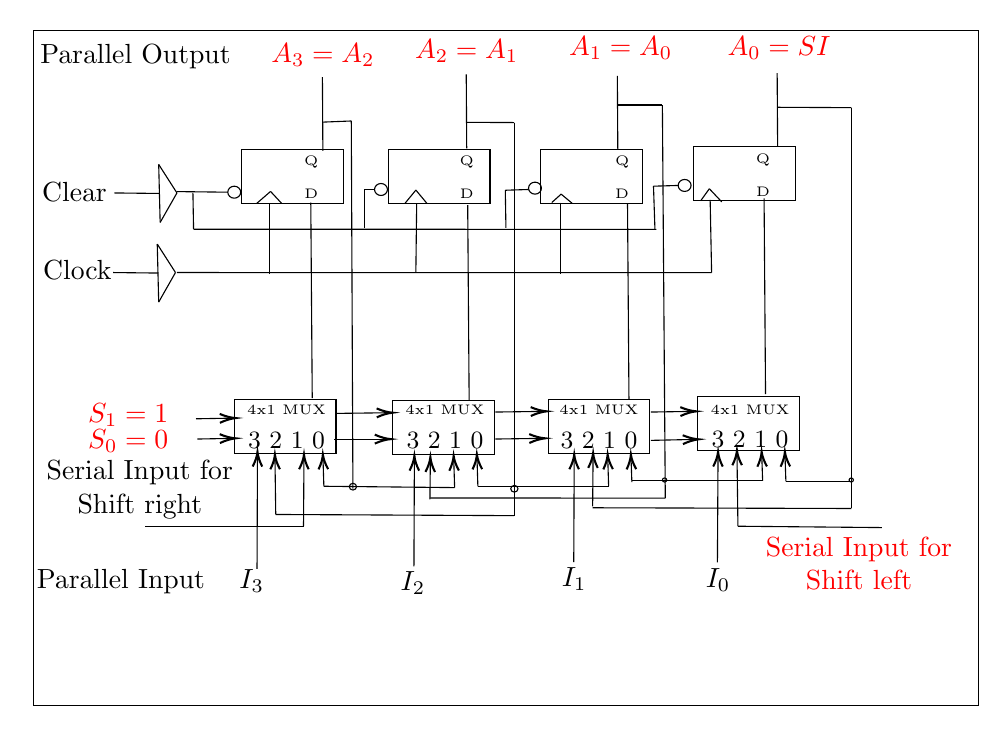
\begin{tikzpicture}[x=0.75pt,y=0.75pt,yscale=-.65,xscale=.7]
   \centering
%uncomment if require: \path (0,482.89410400390625); %set diagram left start at 0, and has height of 482.89410400390625
\draw (0,0) rectangle (650,500);
\draw    (247, 274) rectangle (317, 314)   ;
\draw    (138, 273) rectangle (208, 313)   ;
\draw    (354, 273) rectangle (424, 313)   ;
\draw    (457, 271) rectangle (527, 311)   ;
\draw    (244, 88) rectangle (314, 128)   ;
\draw    (143, 88) rectangle (213, 128)   ;
\draw    (349, 88) rectangle (419, 128)   ;
\draw    (454, 86) rectangle (524, 126)   ;
\draw    (111.68,287.53) -- (137,287.04) ;
\draw [shift={(139,287)}, rotate = 538.88] [color={rgb, 255:red, 0; green, 0; blue, 0 }  ][line width=0.75]    (10.93,-3.29) .. controls (6.95,-1.4) and (3.31,-0.3) .. (0,0) .. controls (3.31,0.3) and (6.95,1.4) .. (10.93,3.29)   ;

\draw    (112.68,302.53) -- (137,302.04) ;
\draw [shift={(139,302)}, rotate = 538.8399999999999] [color={rgb, 255:red, 0; green, 0; blue, 0 }  ][line width=0.75]    (10.93,-3.29) .. controls (6.95,-1.4) and (3.31,-0.3) .. (0,0) .. controls (3.31,0.3) and (6.95,1.4) .. (10.93,3.29)   ;

\draw    (153.68,398.85) -- (153.99,314) ;
\draw [shift={(154,312)}, rotate = 450.21] [color={rgb, 255:red, 0; green, 0; blue, 0 }  ][line width=0.75]    (10.93,-3.29) .. controls (6.95,-1.4) and (3.31,-0.3) .. (0,0) .. controls (3.31,0.3) and (6.95,1.4) .. (10.93,3.29)   ;

\draw    (261.68,396.85) -- (261.99,317) ;
\draw [shift={(262,315)}, rotate = 450.22] [color={rgb, 255:red, 0; green, 0; blue, 0 }  ][line width=0.75]    (10.93,-3.29) .. controls (6.95,-1.4) and (3.31,-0.3) .. (0,0) .. controls (3.31,0.3) and (6.95,1.4) .. (10.93,3.29)   ;

\draw    (371.68,393.85) -- (371.99,316) ;
\draw [shift={(372,314)}, rotate = 450.23] [color={rgb, 255:red, 0; green, 0; blue, 0 }  ][line width=0.75]    (10.93,-3.29) .. controls (6.95,-1.4) and (3.31,-0.3) .. (0,0) .. controls (3.31,0.3) and (6.95,1.4) .. (10.93,3.29)   ;

\draw    (470.56,393.89) -- (470.99,314) ;
\draw [shift={(471,312)}, rotate = 450.31] [color={rgb, 255:red, 0; green, 0; blue, 0 }  ][line width=0.75]    (10.93,-3.29) .. controls (6.95,-1.4) and (3.31,-0.3) .. (0,0) .. controls (3.31,0.3) and (6.95,1.4) .. (10.93,3.29)   ;

\draw    (185.68,367.16) -- (185.99,316) ;
\draw [shift={(186,314)}, rotate = 450.34] [color={rgb, 255:red, 0; green, 0; blue, 0 }  ][line width=0.75]    (10.93,-3.29) .. controls (6.95,-1.4) and (3.31,-0.3) .. (0,0) .. controls (3.31,0.3) and (6.95,1.4) .. (10.93,3.29)   ;

\draw    (76.68,367.16) -- (185.68,367.16) ;


\draw    (484.68,367.16) -- (484.02,313) ;
\draw [shift={(484,311)}, rotate = 449.3] [color={rgb, 255:red, 0; green, 0; blue, 0 }  ][line width=0.75]    (10.93,-3.29) .. controls (6.95,-1.4) and (3.31,-0.3) .. (0,0) .. controls (3.31,0.3) and (6.95,1.4) .. (10.93,3.29)   ;

\draw    (484.68,367.16) -- (583.68,368.16) ;


\draw    (511.68,31.27) -- (512,86) ;


\draw    (401.68,33.27) -- (402,88) ;


\draw    (297.68,32.27) -- (298,87) ;


\draw    (198.68,34.27) -- (199,89) ;


\draw    (562.68,56.9) -- (562.68,333.9) ;


\draw    (517.68,333.9) -- (562.68,333.9) ;


\draw    (511.84,56.63) -- (562.68,56.9) ;


\draw    (517.68,333.9) -- (517.06,314) ;
\draw [shift={(517,312)}, rotate = 448.21] [color={rgb, 255:red, 0; green, 0; blue, 0 }  ][line width=0.75]    (10.93,-3.29) .. controls (6.95,-1.4) and (3.31,-0.3) .. (0,0) .. controls (3.31,0.3) and (6.95,1.4) .. (10.93,3.29)   ;

\draw    (501.68,333.53) -- (501.06,314) ;
\draw [shift={(501,312)}, rotate = 448.18] [color={rgb, 255:red, 0; green, 0; blue, 0 }  ][line width=0.75]    (10.93,-3.29) .. controls (6.95,-1.4) and (3.31,-0.3) .. (0,0) .. controls (3.31,0.3) and (6.95,1.4) .. (10.93,3.29)   ;

\draw    (411.68,334.53) -- (411.07,316) ;
\draw [shift={(411,314)}, rotate = 448.09] [color={rgb, 255:red, 0; green, 0; blue, 0 }  ][line width=0.75]    (10.93,-3.29) .. controls (6.95,-1.4) and (3.31,-0.3) .. (0,0) .. controls (3.31,0.3) and (6.95,1.4) .. (10.93,3.29)   ;

\draw    (411.68,333.53) -- (501.68,333.53) ;


\draw    (562.68,354.01) -- (562.68,333.9) ;


\draw    (384.68,352.48) -- (384.98,315) ;
\draw [shift={(385,313)}, rotate = 450.46] [color={rgb, 255:red, 0; green, 0; blue, 0 }  ][line width=0.75]    (10.93,-3.29) .. controls (6.95,-1.4) and (3.31,-0.3) .. (0,0) .. controls (3.31,0.3) and (6.95,1.4) .. (10.93,3.29)   ;

\draw    (384.68,353.48) -- (562.68,354.01) ;


\draw    (305.68,337.53) -- (395.68,337.53) ;


\draw    (395.68,337.53) -- (395.06,316) ;
\draw [shift={(395,314)}, rotate = 448.33] [color={rgb, 255:red, 0; green, 0; blue, 0 }  ][line width=0.75]    (10.93,-3.29) .. controls (6.95,-1.4) and (3.31,-0.3) .. (0,0) .. controls (3.31,0.3) and (6.95,1.4) .. (10.93,3.29)   ;

\draw    (305.68,337.53) -- (305.06,316) ;
\draw [shift={(305,314)}, rotate = 448.33] [color={rgb, 255:red, 0; green, 0; blue, 0 }  ][line width=0.75]    (10.93,-3.29) .. controls (6.95,-1.4) and (3.31,-0.3) .. (0,0) .. controls (3.31,0.3) and (6.95,1.4) .. (10.93,3.29)   ;

\draw    (289.68,338.53) -- (289.06,317) ;
\draw [shift={(289,315)}, rotate = 448.33] [color={rgb, 255:red, 0; green, 0; blue, 0 }  ][line width=0.75]    (10.93,-3.29) .. controls (6.95,-1.4) and (3.31,-0.3) .. (0,0) .. controls (3.31,0.3) and (6.95,1.4) .. (10.93,3.29)   ;

\draw    (199.68,337.53) -- (199.06,316) ;
\draw [shift={(199,314)}, rotate = 448.33] [color={rgb, 255:red, 0; green, 0; blue, 0 }  ][line width=0.75]    (10.93,-3.29) .. controls (6.95,-1.4) and (3.31,-0.3) .. (0,0) .. controls (3.31,0.3) and (6.95,1.4) .. (10.93,3.29)   ;

\draw    (199.68,337.53) -- (289.68,338.53) ;


\draw    (502.68,124.22) -- (503.68,269.22) ;


\draw    (408.68,128.22) -- (409.68,273.22) ;


\draw    (298.68,129.22) -- (299.68,274.22) ;


\draw    (190.68,127.22) -- (191.68,272.22) ;


\draw    (206.68,302.59) -- (243.68,302.59) ;
\draw [shift={(245.68,302.59)}, rotate = 180] [color={rgb, 255:red, 0; green, 0; blue, 0 }  ][line width=0.75]    (10.93,-3.29) .. controls (6.95,-1.4) and (3.31,-0.3) .. (0,0) .. controls (3.31,0.3) and (6.95,1.4) .. (10.93,3.29)   ;

\draw    (317.68,302.53) -- (350,302.03) ;
\draw [shift={(352,302)}, rotate = 539.11] [color={rgb, 255:red, 0; green, 0; blue, 0 }  ][line width=0.75]    (10.93,-3.29) .. controls (6.95,-1.4) and (3.31,-0.3) .. (0,0) .. controls (3.31,0.3) and (6.95,1.4) .. (10.93,3.29)   ;

\draw    (424.68,303.53) -- (455.68,302.79) ;
\draw [shift={(457.68,302.74)}, rotate = 538.63] [color={rgb, 255:red, 0; green, 0; blue, 0 }  ][line width=0.75]    (10.93,-3.29) .. controls (6.95,-1.4) and (3.31,-0.3) .. (0,0) .. controls (3.31,0.3) and (6.95,1.4) .. (10.93,3.29)   ;

\draw    (208.68,283.53) -- (245,283.03) ;
\draw [shift={(247,283)}, rotate = 539.2] [color={rgb, 255:red, 0; green, 0; blue, 0 }  ][line width=0.75]    (10.93,-3.29) .. controls (6.95,-1.4) and (3.31,-0.3) .. (0,0) .. controls (3.31,0.3) and (6.95,1.4) .. (10.93,3.29)   ;

\draw    (317.68,282.53) -- (351,282.03) ;
\draw [shift={(353,282)}, rotate = 539.14] [color={rgb, 255:red, 0; green, 0; blue, 0 }  ][line width=0.75]    (10.93,-3.29) .. controls (6.95,-1.4) and (3.31,-0.3) .. (0,0) .. controls (3.31,0.3) and (6.95,1.4) .. (10.93,3.29)   ;

\draw    (424.68,282.53) -- (454,282.03) ;
\draw [shift={(456,282)}, rotate = 539.03] [color={rgb, 255:red, 0; green, 0; blue, 0 }  ][line width=0.75]    (10.93,-3.29) .. controls (6.95,-1.4) and (3.31,-0.3) .. (0,0) .. controls (3.31,0.3) and (6.95,1.4) .. (10.93,3.29)   ;

\draw    (272.68,347.22) -- (272.98,318) ;
\draw [shift={(273,316)}, rotate = 450.58] [color={rgb, 255:red, 0; green, 0; blue, 0 }  ][line width=0.75]    (10.93,-3.29) .. controls (6.95,-1.4) and (3.31,-0.3) .. (0,0) .. controls (3.31,0.3) and (6.95,1.4) .. (10.93,3.29)   ;

\draw    (434.68,346.32) -- (272.68,346.22) ;


\draw    (432.68,54.95) -- (434.68,346.32) ;


\draw    (401.68,54.95) -- (432.68,54.95) ;


\draw    (562.68, 332.9) circle [x radius= 1.5, y radius= 1.5]  ;
\draw    (434.18, 332.9) circle [x radius= 1.5, y radius= 1.5]  ;
\draw    (330.68,67.95) -- (330.68,359.32) ;


\draw    (166.56,358.45) -- (166.02,316) ;
\draw [shift={(166,314)}, rotate = 449.28] [color={rgb, 255:red, 0; green, 0; blue, 0 }  ][line width=0.75]    (10.93,-3.29) .. controls (6.95,-1.4) and (3.31,-0.3) .. (0,0) .. controls (3.31,0.3) and (6.95,1.4) .. (10.93,3.29)   ;

\draw    (166.56,358.45) -- (330.68,359.32) ;


\draw    (330.79, 339.39) circle [x radius= 2.5, y radius= 2.5]  ;
\draw    (297.56,67.78) -- (330.68,67.95) ;


\draw    (218.56,66.78) -- (219.68,339.32) ;


\draw    (198.84,67.63) -- (218.56,66.78) ;


\draw    (219.68, 337.84) circle [x radius= 2.5, y radius= 2.5]  ;
\draw    (55.56,120.12) -- (86.5,120.5) ;


\draw    (86,99) -- (98.56,120.12) ;


\draw    (87,142) -- (98.56,120.12) ;


\draw    (86,99) -- (87,142) ;


\draw    (138, 119.56) circle [x radius= 4.44, y radius= 4.44]  ;
\draw    (239, 117.56) circle [x radius= 4.44, y radius= 4.44]  ;
\draw    (345, 116.56) circle [x radius= 4.44, y radius= 4.44]  ;
\draw    (448, 114.56) circle [x radius= 4.44, y radius= 4.44]  ;
\draw    (98.56,119.12) -- (133.56,119.56) ;


\draw    (110,147) -- (428.56,147.12) ;


\draw    (110,147) -- (109.56,120.12) ;


\draw    (227.56,117.56) -- (227.56,146.12) ;


\draw    (227.56,117.56) -- (234.56,117.56) ;


\draw    (325,146) -- (324.56,118.12) ;


\draw    (324.56,118.12) -- (340.56,117.56) ;


\draw    (427.56,147.12) -- (426.56,115.12) ;


\draw    (426.56,115.12) -- (443.56,114.56) ;


\draw    (54.56,179.12) -- (85.5,179.5) ;


\draw    (85,158) -- (97.56,179.12) ;


\draw    (86,201) -- (97.56,179.12) ;


\draw    (85,158) -- (86,201) ;


\draw    (98.56,179.12) -- (466.56,179.23) ;


%\draw    (102.56, 179.12) circle [x radius= 5, y radius= 5]  ;
\draw    (465.56,125.23) -- (466.56,179.23) ;


\draw    (362.56,127.23) -- (362.56,180.23) ;


\draw    (263.56,128.23) -- (263,179) ;


\draw    (162,128) -- (162,180) ;


\draw    (163,119) -- (170.56,127.78) ;


\draw    (163,119) -- (153.56,127.78) ;


\draw    (263,118) -- (270.56,127.78) ;


\draw    (263,118) -- (255.56,127.78) ;


\draw    (363,121) -- (370.56,127.78) ;


\draw    (363,121) -- (356.56,127.23) ;


\draw    (465,117) -- (473.56,126.78) ;


\draw    (465,117) -- (459,126) ;



\draw (150,408) node  [align=center] {$I_3$};
\draw (261,409) node  [align=center] {$I_2$};
\draw (372,406) node [align=center]{$I_1$};
\draw (471,407) node [align=center] {$I_0$};
\draw (73,340) node  [align=center] {Serial Input for\\Shift right};
\draw (568,395) node  [align=center,color=red] {Serial Input for\\Shift left};
\draw (65,285) node  [align=center,color=red] {$S_1=1$};
\draw (65,304) node [align=center,color=red] {$S_0=0$};
\draw (199,18) node  [align=center,color=red] {$A_3=A_2$};
\draw (298,15) node  [align=center,color=red] {$A_2=A_1$};
\draw (404,13) node  [align=center,color=red] {$A_1=A_0$};
\draw (513,13) node  [align=center,color=red] {$A_0=SI$};
\draw (60,408) node  [align=center] {Parallel Input};
\draw (70,19) node  [align=center] {Parallel Output};
\draw (28,119) node  [align=center] {Clear};
\draw (30,177) node  [align=center] {Clock};
\draw (191,108.5) node  [align=center] {\tiny Q\\\tiny D};
\draw (298,108.5) node  [align=center] {\tiny Q\\\tiny D};
\draw (405,108.5) node  [align=center] {\tiny Q\\\tiny D};
\draw (502,107) node  [align=center] {\tiny Q\\\tiny D};
\draw (174,293.5) node [align=center] {\tiny 4x1 MUX\\\small 3 2 1 0};
\draw (283,293.5) node  [align=center] {\tiny 4x1 MUX\\\small 3 2 1 0};
\draw (389,293.5) node  [align=center] {\tiny 4x1 MUX\\\small 3 2 1 0};
\draw (493,293) node  [align=center] {\tiny 4x1 MUX\\\small 3 2 1 0};


\end{tikzpicture}
    \caption{Left shifting data by universal shift register}
    \label{fig:leftshift}
\end{figure}
We can see from the figure that,outputs of the universal shift register will be shifted left if selection bits, $S_1=1$ and $S_0=0$.This configuration can be used for serial communication between electrical devices.
\subsection{Parallel Loading}
Data can be parallelly loaded by universal shift register.When $S_1=1$ and $S_0=1$ the outputs of the universal shift register will be parallelly loaded from parallel inputs.\newpage
\begin{figure}[!ht]
    \centering
\tikzset{every picture/.style={line width=0.75pt}} %set default line width to 0.75pt        

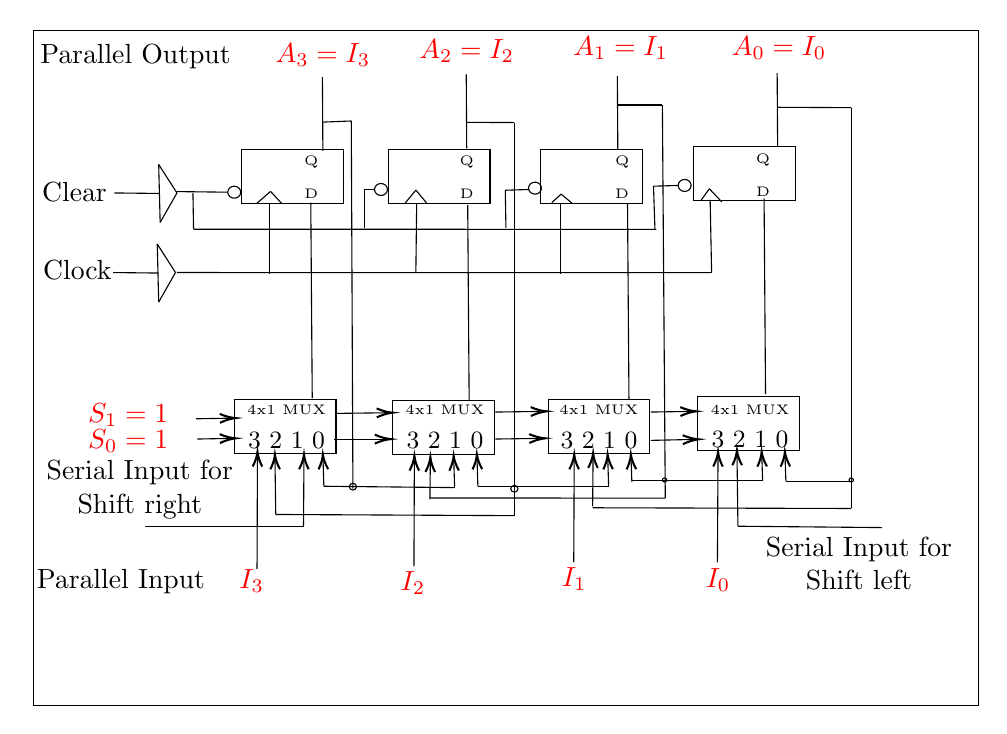
\begin{tikzpicture}[x=0.75pt,y=0.75pt,yscale=-.65,xscale=.7]
   \centering
%uncomment if require: \path (0,482.89410400390625); %set diagram left start at 0, and has height of 482.89410400390625
\draw (0,0) rectangle (650,500);
\draw    (247, 274) rectangle (317, 314)   ;
\draw    (138, 273) rectangle (208, 313)   ;
\draw    (354, 273) rectangle (424, 313)   ;
\draw    (457, 271) rectangle (527, 311)   ;
\draw    (244, 88) rectangle (314, 128)   ;
\draw    (143, 88) rectangle (213, 128)   ;
\draw    (349, 88) rectangle (419, 128)   ;
\draw    (454, 86) rectangle (524, 126)   ;
\draw    (111.68,287.53) -- (137,287.04) ;
\draw [shift={(139,287)}, rotate = 538.88] [color={rgb, 255:red, 0; green, 0; blue, 0 }  ][line width=0.75]    (10.93,-3.29) .. controls (6.95,-1.4) and (3.31,-0.3) .. (0,0) .. controls (3.31,0.3) and (6.95,1.4) .. (10.93,3.29)   ;

\draw    (112.68,302.53) -- (137,302.04) ;
\draw [shift={(139,302)}, rotate = 538.8399999999999] [color={rgb, 255:red, 0; green, 0; blue, 0 }  ][line width=0.75]    (10.93,-3.29) .. controls (6.95,-1.4) and (3.31,-0.3) .. (0,0) .. controls (3.31,0.3) and (6.95,1.4) .. (10.93,3.29)   ;

\draw    (153.68,398.85) -- (153.99,314) ;
\draw [shift={(154,312)}, rotate = 450.21] [color={rgb, 255:red, 0; green, 0; blue, 0 }  ][line width=0.75]    (10.93,-3.29) .. controls (6.95,-1.4) and (3.31,-0.3) .. (0,0) .. controls (3.31,0.3) and (6.95,1.4) .. (10.93,3.29)   ;

\draw    (261.68,396.85) -- (261.99,317) ;
\draw [shift={(262,315)}, rotate = 450.22] [color={rgb, 255:red, 0; green, 0; blue, 0 }  ][line width=0.75]    (10.93,-3.29) .. controls (6.95,-1.4) and (3.31,-0.3) .. (0,0) .. controls (3.31,0.3) and (6.95,1.4) .. (10.93,3.29)   ;

\draw    (371.68,393.85) -- (371.99,316) ;
\draw [shift={(372,314)}, rotate = 450.23] [color={rgb, 255:red, 0; green, 0; blue, 0 }  ][line width=0.75]    (10.93,-3.29) .. controls (6.95,-1.4) and (3.31,-0.3) .. (0,0) .. controls (3.31,0.3) and (6.95,1.4) .. (10.93,3.29)   ;

\draw    (470.56,393.89) -- (470.99,314) ;
\draw [shift={(471,312)}, rotate = 450.31] [color={rgb, 255:red, 0; green, 0; blue, 0 }  ][line width=0.75]    (10.93,-3.29) .. controls (6.95,-1.4) and (3.31,-0.3) .. (0,0) .. controls (3.31,0.3) and (6.95,1.4) .. (10.93,3.29)   ;

\draw    (185.68,367.16) -- (185.99,316) ;
\draw [shift={(186,314)}, rotate = 450.34] [color={rgb, 255:red, 0; green, 0; blue, 0 }  ][line width=0.75]    (10.93,-3.29) .. controls (6.95,-1.4) and (3.31,-0.3) .. (0,0) .. controls (3.31,0.3) and (6.95,1.4) .. (10.93,3.29)   ;

\draw    (76.68,367.16) -- (185.68,367.16) ;


\draw    (484.68,367.16) -- (484.02,313) ;
\draw [shift={(484,311)}, rotate = 449.3] [color={rgb, 255:red, 0; green, 0; blue, 0 }  ][line width=0.75]    (10.93,-3.29) .. controls (6.95,-1.4) and (3.31,-0.3) .. (0,0) .. controls (3.31,0.3) and (6.95,1.4) .. (10.93,3.29)   ;

\draw    (484.68,367.16) -- (583.68,368.16) ;


\draw    (511.68,31.27) -- (512,86) ;


\draw    (401.68,33.27) -- (402,88) ;


\draw    (297.68,32.27) -- (298,87) ;


\draw    (198.68,34.27) -- (199,89) ;


\draw    (562.68,56.9) -- (562.68,333.9) ;


\draw    (517.68,333.9) -- (562.68,333.9) ;


\draw    (511.84,56.63) -- (562.68,56.9) ;


\draw    (517.68,333.9) -- (517.06,314) ;
\draw [shift={(517,312)}, rotate = 448.21] [color={rgb, 255:red, 0; green, 0; blue, 0 }  ][line width=0.75]    (10.93,-3.29) .. controls (6.95,-1.4) and (3.31,-0.3) .. (0,0) .. controls (3.31,0.3) and (6.95,1.4) .. (10.93,3.29)   ;

\draw    (501.68,333.53) -- (501.06,314) ;
\draw [shift={(501,312)}, rotate = 448.18] [color={rgb, 255:red, 0; green, 0; blue, 0 }  ][line width=0.75]    (10.93,-3.29) .. controls (6.95,-1.4) and (3.31,-0.3) .. (0,0) .. controls (3.31,0.3) and (6.95,1.4) .. (10.93,3.29)   ;

\draw    (411.68,334.53) -- (411.07,316) ;
\draw [shift={(411,314)}, rotate = 448.09] [color={rgb, 255:red, 0; green, 0; blue, 0 }  ][line width=0.75]    (10.93,-3.29) .. controls (6.95,-1.4) and (3.31,-0.3) .. (0,0) .. controls (3.31,0.3) and (6.95,1.4) .. (10.93,3.29)   ;

\draw    (411.68,333.53) -- (501.68,333.53) ;


\draw    (562.68,354.01) -- (562.68,333.9) ;


\draw    (384.68,352.48) -- (384.98,315) ;
\draw [shift={(385,313)}, rotate = 450.46] [color={rgb, 255:red, 0; green, 0; blue, 0 }  ][line width=0.75]    (10.93,-3.29) .. controls (6.95,-1.4) and (3.31,-0.3) .. (0,0) .. controls (3.31,0.3) and (6.95,1.4) .. (10.93,3.29)   ;

\draw    (384.68,353.48) -- (562.68,354.01) ;


\draw    (305.68,337.53) -- (395.68,337.53) ;


\draw    (395.68,337.53) -- (395.06,316) ;
\draw [shift={(395,314)}, rotate = 448.33] [color={rgb, 255:red, 0; green, 0; blue, 0 }  ][line width=0.75]    (10.93,-3.29) .. controls (6.95,-1.4) and (3.31,-0.3) .. (0,0) .. controls (3.31,0.3) and (6.95,1.4) .. (10.93,3.29)   ;

\draw    (305.68,337.53) -- (305.06,316) ;
\draw [shift={(305,314)}, rotate = 448.33] [color={rgb, 255:red, 0; green, 0; blue, 0 }  ][line width=0.75]    (10.93,-3.29) .. controls (6.95,-1.4) and (3.31,-0.3) .. (0,0) .. controls (3.31,0.3) and (6.95,1.4) .. (10.93,3.29)   ;

\draw    (289.68,338.53) -- (289.06,317) ;
\draw [shift={(289,315)}, rotate = 448.33] [color={rgb, 255:red, 0; green, 0; blue, 0 }  ][line width=0.75]    (10.93,-3.29) .. controls (6.95,-1.4) and (3.31,-0.3) .. (0,0) .. controls (3.31,0.3) and (6.95,1.4) .. (10.93,3.29)   ;

\draw    (199.68,337.53) -- (199.06,316) ;
\draw [shift={(199,314)}, rotate = 448.33] [color={rgb, 255:red, 0; green, 0; blue, 0 }  ][line width=0.75]    (10.93,-3.29) .. controls (6.95,-1.4) and (3.31,-0.3) .. (0,0) .. controls (3.31,0.3) and (6.95,1.4) .. (10.93,3.29)   ;

\draw    (199.68,337.53) -- (289.68,338.53) ;


\draw    (502.68,124.22) -- (503.68,269.22) ;


\draw    (408.68,128.22) -- (409.68,273.22) ;


\draw    (298.68,129.22) -- (299.68,274.22) ;


\draw    (190.68,127.22) -- (191.68,272.22) ;


\draw    (206.68,302.59) -- (243.68,302.59) ;
\draw [shift={(245.68,302.59)}, rotate = 180] [color={rgb, 255:red, 0; green, 0; blue, 0 }  ][line width=0.75]    (10.93,-3.29) .. controls (6.95,-1.4) and (3.31,-0.3) .. (0,0) .. controls (3.31,0.3) and (6.95,1.4) .. (10.93,3.29)   ;

\draw    (317.68,302.53) -- (350,302.03) ;
\draw [shift={(352,302)}, rotate = 539.11] [color={rgb, 255:red, 0; green, 0; blue, 0 }  ][line width=0.75]    (10.93,-3.29) .. controls (6.95,-1.4) and (3.31,-0.3) .. (0,0) .. controls (3.31,0.3) and (6.95,1.4) .. (10.93,3.29)   ;

\draw    (424.68,303.53) -- (455.68,302.79) ;
\draw [shift={(457.68,302.74)}, rotate = 538.63] [color={rgb, 255:red, 0; green, 0; blue, 0 }  ][line width=0.75]    (10.93,-3.29) .. controls (6.95,-1.4) and (3.31,-0.3) .. (0,0) .. controls (3.31,0.3) and (6.95,1.4) .. (10.93,3.29)   ;

\draw    (208.68,283.53) -- (245,283.03) ;
\draw [shift={(247,283)}, rotate = 539.2] [color={rgb, 255:red, 0; green, 0; blue, 0 }  ][line width=0.75]    (10.93,-3.29) .. controls (6.95,-1.4) and (3.31,-0.3) .. (0,0) .. controls (3.31,0.3) and (6.95,1.4) .. (10.93,3.29)   ;

\draw    (317.68,282.53) -- (351,282.03) ;
\draw [shift={(353,282)}, rotate = 539.14] [color={rgb, 255:red, 0; green, 0; blue, 0 }  ][line width=0.75]    (10.93,-3.29) .. controls (6.95,-1.4) and (3.31,-0.3) .. (0,0) .. controls (3.31,0.3) and (6.95,1.4) .. (10.93,3.29)   ;

\draw    (424.68,282.53) -- (454,282.03) ;
\draw [shift={(456,282)}, rotate = 539.03] [color={rgb, 255:red, 0; green, 0; blue, 0 }  ][line width=0.75]    (10.93,-3.29) .. controls (6.95,-1.4) and (3.31,-0.3) .. (0,0) .. controls (3.31,0.3) and (6.95,1.4) .. (10.93,3.29)   ;

\draw    (272.68,347.22) -- (272.98,318) ;
\draw [shift={(273,316)}, rotate = 450.58] [color={rgb, 255:red, 0; green, 0; blue, 0 }  ][line width=0.75]    (10.93,-3.29) .. controls (6.95,-1.4) and (3.31,-0.3) .. (0,0) .. controls (3.31,0.3) and (6.95,1.4) .. (10.93,3.29)   ;

\draw    (434.68,346.32) -- (272.68,346.22) ;


\draw    (432.68,54.95) -- (434.68,346.32) ;


\draw    (401.68,54.95) -- (432.68,54.95) ;


\draw    (562.68, 332.9) circle [x radius= 1.5, y radius= 1.5]  ;
\draw    (434.18, 332.9) circle [x radius= 1.5, y radius= 1.5]  ;
\draw    (330.68,67.95) -- (330.68,359.32) ;


\draw    (166.56,358.45) -- (166.02,316) ;
\draw [shift={(166,314)}, rotate = 449.28] [color={rgb, 255:red, 0; green, 0; blue, 0 }  ][line width=0.75]    (10.93,-3.29) .. controls (6.95,-1.4) and (3.31,-0.3) .. (0,0) .. controls (3.31,0.3) and (6.95,1.4) .. (10.93,3.29)   ;

\draw    (166.56,358.45) -- (330.68,359.32) ;


\draw    (330.79, 339.39) circle [x radius= 2.5, y radius= 2.5]  ;
\draw    (297.56,67.78) -- (330.68,67.95) ;


\draw    (218.56,66.78) -- (219.68,339.32) ;


\draw    (198.84,67.63) -- (218.56,66.78) ;


\draw    (219.68, 337.84) circle [x radius= 2.5, y radius= 2.5]  ;
\draw    (55.56,120.12) -- (86.5,120.5) ;


\draw    (86,99) -- (98.56,120.12) ;


\draw    (87,142) -- (98.56,120.12) ;


\draw    (86,99) -- (87,142) ;


\draw    (138, 119.56) circle [x radius= 4.44, y radius= 4.44]  ;
\draw    (239, 117.56) circle [x radius= 4.44, y radius= 4.44]  ;
\draw    (345, 116.56) circle [x radius= 4.44, y radius= 4.44]  ;
\draw    (448, 114.56) circle [x radius= 4.44, y radius= 4.44]  ;
\draw    (98.56,119.12) -- (133.56,119.56) ;


\draw    (110,147) -- (428.56,147.12) ;


\draw    (110,147) -- (109.56,120.12) ;


\draw    (227.56,117.56) -- (227.56,146.12) ;


\draw    (227.56,117.56) -- (234.56,117.56) ;


\draw    (325,146) -- (324.56,118.12) ;


\draw    (324.56,118.12) -- (340.56,117.56) ;


\draw    (427.56,147.12) -- (426.56,115.12) ;


\draw    (426.56,115.12) -- (443.56,114.56) ;


\draw    (54.56,179.12) -- (85.5,179.5) ;


\draw    (85,158) -- (97.56,179.12) ;


\draw    (86,201) -- (97.56,179.12) ;


\draw    (85,158) -- (86,201) ;


\draw    (98.56,179.12) -- (466.56,179.23) ;


%\draw    (102.56, 179.12) circle [x radius= 5, y radius= 5]  ;
\draw    (465.56,125.23) -- (466.56,179.23) ;


\draw    (362.56,127.23) -- (362.56,180.23) ;


\draw    (263.56,128.23) -- (263,179) ;


\draw    (162,128) -- (162,180) ;


\draw    (163,119) -- (170.56,127.78) ;


\draw    (163,119) -- (153.56,127.78) ;


\draw    (263,118) -- (270.56,127.78) ;


\draw    (263,118) -- (255.56,127.78) ;


\draw    (363,121) -- (370.56,127.78) ;


\draw    (363,121) -- (356.56,127.23) ;


\draw    (465,117) -- (473.56,126.78) ;


\draw    (465,117) -- (459,126) ;



\draw (150,408) node  [align=center,color=red] {$I_3$};
\draw (261,409) node  [align=center,color=red] {$I_2$};
\draw (372,406) node [align=center,color=red]{$I_1$};
\draw (471,407) node [align=center,color=red] {$I_0$};
\draw (73,340) node  [align=center] {Serial Input for\\Shift right};
\draw (568,395) node  [align=center] {Serial Input for\\Shift left};
\draw (65,285) node  [align=center,color=red] {$S_1=1$};
\draw (65,304) node [align=center,color=red] {$S_0=1$};
\draw (199,18) node  [align=center,color=red] {$A_3=I_3$};
\draw (298,15) node  [align=center,color=red] {$A_2=I_2$};
\draw (404,13) node  [align=center,color=red] {$A_1=I_1$};
\draw (513,13) node  [align=center,color=red] {$A_0=I_0$};
\draw (60,408) node  [align=center] {Parallel Input};
\draw (70,19) node  [align=center] {Parallel Output};
\draw (28,119) node  [align=center] {Clear};
\draw (30,177) node  [align=center] {Clock};
\draw (191,108.5) node  [align=center] {\tiny Q\\\tiny D};
\draw (298,108.5) node  [align=center] {\tiny Q\\\tiny D};
\draw (405,108.5) node  [align=center] {\tiny Q\\\tiny D};
\draw (502,107) node  [align=center] {\tiny Q\\\tiny D};
\draw (174,293.5) node [align=center] {\tiny 4x1 MUX\\\small 3 2 1 0};
\draw (283,293.5) node  [align=center] {\tiny 4x1 MUX\\\small 3 2 1 0};
\draw (389,293.5) node  [align=center] {\tiny 4x1 MUX\\\small 3 2 1 0};
\draw (493,293) node  [align=center] {\tiny 4x1 MUX\\\small 3 2 1 0};


\end{tikzpicture}
    \caption{Parallel loading data by universal shift register}
    \label{fig:parralelload}
\end{figure}
We can see from the figure that,outputs of the universal shift register will be parallelly loaded from parallel input if selection bits, $S_1=1$ and $S_0=1$.This configuration can be used for transferring data.
\section{Uses of Universal Shift Register}
We can use \textbf{Universal Shift Register} in different purposes : \\
\begin{itemize}
\item Temporary data storage
\item Data transfer
\item Data manipulation
\item As counters.
\item Serial communication of micro controller unit
\item Multiplying binary numbers
\item Storing  ALU's operands, intermediate results and final results
\end{itemize}
\section{Conclusion}
Universal shift register is very useful for transferring data, storing and for serial communication.We can use it instead of individual shift register, D flip-flop.In practical use, IC 74194 (4 bit), IC 74198 (8 bit) are used in various devices that receive serial format data. Though now a days it is being replaced by more advanced chips, universal shift register still has great importance in the field of electronics.
\end{flushleft}

\end{document}

